\documentclass[lettersize,journal]{IEEEtran}
\usepackage{amsmath,amsfonts}
\usepackage{amsthm}
\usepackage{algorithmic}
\usepackage{algorithm}
\usepackage{array}
\usepackage[caption=false,font=normalsize,labelfont=sf,textfont=sf]{subfig}
\usepackage{textcomp}
\usepackage{stfloats}
\usepackage{url}
\usepackage{verbatim}
\usepackage{graphicx}
\usepackage{cite}
\usepackage{multirow}
\usepackage{amssymb}
\hyphenation{op-tical net-works semi-conduc-tor IEEE-Xplore}
% updated with editorial comments 8/9/2021

% Lemma style: italic heading/body, proof body in upright roman.
\newtheoremstyle{italiclemma}
  {3pt}{3pt}% Space above/below
  {\itshape}% Body font
  {}% Indent amount
  {\itshape}% Theorem head font
  {.}% Punctuation after theorem head
  {0.5em}% Space after theorem head
  {}% Theorem head spec
\theoremstyle{italiclemma}
\newtheorem{lemma}{Lemma}
\theoremstyle{italictheorem}
\newtheorem{theorem}{Theorem}
\theoremstyle{definition}
\newtheorem{definition}{Definition}
\newtheorem{example}{Example}
\newtheorem{problem}{Problem}[section]
 
\begin{document}

\title{On-the-Fly Temporal-Logic Task Allocation for Heterogeneous Multi-Robot Systems during B\"uchi Automaton Generation }

% \title{Automaton-Construction-Integrated Temporal-Logic Task Allocation for Heterogeneous Multi-Robot Systems }

\author{IEEE Publication Technology,~\IEEEmembership{Staff,~IEEE,}
        % <-this % stops a space
\thanks{This paper was produced by the IEEE Publication Technology Group. They are in Piscataway, NJ.}% <-this % stops a space
\thanks{Manuscript received April 19, 2021; revised August 16, 2021.}}

% The paper headers
\markboth{Journal of \LaTeX\ Class Files,~Vol.~14, No.~8, August~2021}%
{Shell \MakeLowercase{\textit{et al.}}: A Sample Article Using IEEEtran.cls for IEEE Journals}

\IEEEpubid{0000--0000/00\$00.00~\copyright~2021 IEEE}
% Remember, if you use this you must call \IEEEpubidadjcol in the second
% column for its text to clear the IEEEpubid mark.

\maketitle

\begin{abstract}


This paper studies multi-robot task allocation under global linear temporal logic (LTL) specifications for heterogeneous robot teams. Existing methods typically construct the complete automaton before performing task allocation, which can delay the first feasible solution in large-scale problems and hinder rapid plan repair when robot availability changes during execution. To address these limitations, we propose an on-the-fly framework that performs temporal-logic task allocation within Büchi automaton generation. The method prunes infeasible and redundant transitions during generalized Büchi automaton construction, and then  synchronously builds a nondeterministic Büchi automaton and a  plan graph.
The method prunes infeasible and redundant transitions during generalized Büchi automaton construction, and then  synchronously builds a nondeterministic Büchi automaton and a plan graph.
Once an accepting prefix-suffix structure is reached, the framework can immediately return an initial executable plan. After the plan graph is fully constructed, a feasible solution extracted from the completed graph is used to warm-start a branch-and-bound optimizer for further improvement. The same  workflow is also used to repair the remaining mission when robots become unavailable during execution. Theoretical analysis establishes completeness of the proposed framework. The proposed framework is validated through extensive numerical simulations against strong baselines and hardware experiments. The results demonstrate that it generates feasible plans much faster in large-scale systems with complex LTL specifications, while also maintaining rapid plan repair when robots become unavailable during online execution.
\end{abstract}

\begin{IEEEkeywords}
Linear temporal logic, multi-robot task allocation, heterogeneous robots, anytime search.
\end{IEEEkeywords}

\section{INTRODUCTION}

Multi-robot systems (MRS) have been widely used in applications such as persistent surveillance\cite{leahy2016persistent}, logistics\cite{LiRAL23}, and autonomous maintenance\cite{liu2024time}, where multiple robots can operate concurrently and cooperatively to improve efficiency and accomplish tasks that are beyond the capability of a single robot. In practice, many multi-robot tasks are subject to temporal requirements. For instance, in a smart factory or large warehouse, carriers may first transport tools or shelves to a target region, inspection robots may verify safety conditions before manipulation begins, and monitoring robots may be required to continuously patrol surrounding areas. Such task dependencies naturally introduce temporal constraints such as ordering, persistence, and synchronization. To specify these constraints in a rigorous way, many recent work have used formal languages such as linear temporal logic (LTL)\cite{baier2008principles}; see, for example,\cite{schillinger2018decomposition, 11441465}. 


% 问题难点，不要展开文献细节

% 这一段不要进入“某某文献做了什么”，而是抽象总结困难。

% 建议你写 3 个难点：

% 任务分配组合爆炸；
% 自动机/规划结构随任务复杂度迅速膨胀；
% 既要尽快给首个可行解，又希望继续优化到最优，这两者常常冲突。

% 这里可以借鉴 Luo 对 product graph 复杂性的概括，以及 Liu 对实际需求中“实时性”与“同步/在线适应”重要性的提炼。
In this work, we consider the multi-robot task allocation (MRTA) problem under temporal logic specifications, referred to as LTL-MRTA, which was formalized in \cite{luo2022temporal}. In LTL-MRTA, the task is specified by an LTL formula, but the specific robots assigned to each subtask are not predetermined by the formula. For example, . For example, a specification may require two type-1 robots to complete a pickup-and-delivery task before waiting at the delivery site until a type-2 robot arrives, without prescribing which individual robots should execute these subtasks. This problem becomes increasingly difficult as the number of robots and the complexity of the task specification grow, since the associated search and optimization space may expand explosively. As a result, existing approaches, such as mixed-integer linear programming (MILP)-based methods\cite{luo2022temporal, 9663414} and search-based methods \cite{ulusoy2013optimality, kantaros2020stylus} can be computationally demanding in large-scale problems, even when only an initial feasible solution is required. 

In practical robotic applications, however, it is often important to obtain an executable solution early, especially in large-scale settings where task execution needs to start promptly and decisions may need to be updated online.  Planning-tree-based \cite{Chen2024RealTimeReactive,11441465} and partial-order-based methods \cite{liu2024time} highlighted the practical importance of fast first-solution generation. However, planning-tree-based methods may be prone to local optima, while partial-order-based methods may be less effective for complex tasks due to the need to extract the partial-order relations among subtasks. Consequently, for LTL-MRTA, developing methods that can quickly return a feasible solution and further improve it toward optimality remains an important research direction. In real-robot execution, the available team may also change unexpectedly due to hardware faults, robot damage, localization failures, or battery depletion. Such events do not necessarily change the temporal-logic mission itself, but they invalidate assignments involving the unavailable robots and require the remaining mission to be repaired from the current execution state. Therefore, an LTL-MRTA planner should not only generate an executable plan before execution, but also support fast online replanning when the available robot set changes.



% 方法总览，必须像 Luo 一样写成 pipeline

% 这一段要学 Luo 最多。
% 不要拆成三个孤立技巧，而要写成连续流程：

% 在自动机构造阶段前置引入机器人系统、环境和规划相关信息；
% 在 GBA 生成中进行可行性剪枝和可分解性剪枝，提前排除对当前系统无意义的分支；
% 在 NBA 生成阶段进一步结合规划信息，仅保留与后续求解相关的结构；
% 基于生成的规划树采用热启动分支定界；
% 因此实现“更快首解 + 最终最优”。

% Luo 那篇就是这样：先 prune/relax NBA，再提 subtasks 和 temporal orders，再做高层分配，再做可执行路径。这个“流水线感”非常强。
To address this problem, we propose a novel framework that integrates robot planning into the automaton generation process. Unlike existing methods that first construct the complete NBA and then perform planning on top of it, our approach introduces information about the robot team, the workspace, and intermediate planning results during the translation from LTL to automata. Specifically, we follow the translation pipeline of LTL2BA\cite{Gastin2001FastLT}, a classical tool widely used in the literature\cite{10530927,schillinger2018simultaneous}, which translates an LTL formula into a very weak alternating automaton (VWAA), then into a generalized Büchi automaton (GBA), and finally into a nondeterministic Büchi automaton (NBA). During GBA construction, each candidate transition is screened before insertion against the robot types and cardinalities available in the team, and candidates whose simultaneous action requirements cannot be satisfied are discarded. After the GBA is constructed,  transitions that impose unnecessary synchronization are removed.
During NBA generation, each newly generated transition induces a subtask. A greedy task-allocation procedure is then applied to the induced subtask. The feasible assignment is recorded in a plan graph. Consequently, an executable plan becomes available as soon as an accepting prefix--suffix structure is generated, before the complete NBA has been constructed. After the plan graph has been completed, the executable plan initializes the incumbent of a branch-and-bound optimizer. When a robot becomes unavailable during execution, the method re-roots the retained plan graph at the last confirmed execution state and re-optimizes the unfinished assignments over the surviving team. In this way, the proposed method supports rapid first-solution generation as well as continued improvement toward better solutions. 

\subsection{Related Work}
% 先总起讲大概背景
Existing  planning methods under LTL constraints can generally be classified into bottom-up and top-down  approaches. Bottom-up approaches usually formulate the problem as a task-coordination problem under local LTL specifications, where each robot is assigned a local LTL task and team behavior is achieved through communication, synchronization, and online replanning. For example, Guo et al.\cite{guo2015multi} studied a decentralized planning framework under local LTL specifications with online plan reconfiguration, while Yu et al. \cite{2022Distributed} developed a distributed motion-coordination strategy under local LTL specifications, where conflicts among neighboring robots are detected and resolved online to ensure safety and task satisfaction. In contrast, top-down approaches start from a global LTL formula that specifies the overall team mission. This paper focuses on the latter setting.

For top-down methods, a common strategy is to construct the product automaton of  NBA translated from the global LTL formula and the discrete transition systems of the robots and then solve the resulting graph-search problem \cite{smith2010optimal,ulusoy2013optimality}.  However, this approach suffers from state explosion , because the number of states in the product automaton increases rapidly with the workspace/state-space size, the number of robots, and the complexity of the task, as reflected by the size of the automaton derived from the specification. To alleviate this issue, sampling-based methods \cite{kantaros2020stylus,kantaros2018sampling} incrementally construct trees that approximate the state space and transitions of the synchronous product automaton, instead of explicitly building the full product automaton. This significantly improves scalability while retaining probabilistic completeness and asymptotic optimality. However, such methods typically require the global LTL formula to explicitly assign subtasks to robots. When the robot assignment is not given a priori, a possible workaround is to enumerate all admissible robot combinations and connect them using OR operators, but this can result in exponentially long LTL formulas. 

To avoid the combinatorial burden and reduced flexibility caused by explicitly allocate tasks to robots, some works decompose the global LTL specifications. For example, \cite{schillinger2017multi,schillinger2018simultaneous} proposed the simultaneous task allocation and planning (STAP) framework, which constructs a team model that integrates task decomposition and task allocation. By decomposing the global task into parallelizable subtasks, the framework improves planning efficiency. However, these works do not explicitly address tightly coupled collaborative tasks requiring the simultaneous participation of multiple robots. Other works address global temporal-logic task planning by using mixed-integer linear programming (MILP)\cite{luo2022temporal,karaman2008vehicle,9663414}.  In particular, to mitigate the impact of workspace size on the computational burden, \cite{luo2022temporal} proposed a hierarchical architecture that separates task planning from motion planning. Unfortunately,  MILP-based methods can become computationally demanding in large-scale settings, even when only a first feasible solution is required. 

Planning-decision-tree-based methods\cite{Chen2024RealTimeReactive, 2025Task } have been proposed to improve the speed of temporal-logic mission planning. These methods represents task progression and task allocation incrementally, enabling real-time planning for large-scale multi-robot systems. Although such methods are highly efficient in generating feasible solutions, they typically rely on greedy task-allocation decisions, and therefore can be prone to getting trapped in local optima. Liu et al.\cite{liu2024time} analyze the task automaton to extract partial-order relations among subtasks, and then use a branch-and-bound search procedure to compute task assignments. Their method explicitly emphasizes the importance of obtaining a valid plan early: it is formulated as an anytime algorithm, so that a feasible solution can be returned quickly and then progressively improved as computation continues. However, when the task specification becomes more complex, the efficiency of obtaining the first feasible solution may decrease, since extracting the partial-order relations among subtasks can itself take additional time. As illustrated in the paper, for an automaton with hundreds of states, the algorithm may require tens or even hundreds of seconds to obtain the first partial order. Some work reduces the burden of complex specifications by changing or exploiting the structure of the task formula. Hierarchical temporal-logic specifications \cite{luo2025simultaneous} organize complex specifications into a hierarchy. Liu et al.\cite{research0337} exploit the case where an sc-LTL mission is given as a conjunc-tion of subformulas; each subformula is converted into a poset and the products of these posets are computed online to accommodate newly released tasks. These methods reduce the burden of complex specifications mainly by changing or exploiting the modeled structure of the LTL specification. While effective, this perspective may require the mission to be expressed in a suitable hierarchical, conjunctive, or otherwise structured form, and shift part of the complexity to specification design or task decomposition.

Overall, while existing top-down methods have advanced LTL-MRTA from different perspectives, they still struggle to simultaneously achieve rapid first-solution generation and effective subsequent optimization in large-scale problems. This limitation is particularly evident when substantial computation is required before a planning structure suitable for allocation can even be obtained. Instead of constructing the complete NBA first and then solving the allocation problem on top of it, the proposed method incorporates robot-team feasibility,
workspace travel information, and partial planning results into the LTL-to-automaton translation process. During GBA construction, infeasible or decomposition-inducing transitions are pruned before they are propagated to the NBA stage. 
During the NBA construction stage, the NBA and a shared directed planning graph are generated synchronously. Whenever a new automaton transition becomes available, the corresponding transition is evaluated by a greedy executable assignment, and newly discovered successor NBA states are ordered within the current pending batch by a lightweight residual-obligation score. Once an accepting prefix-suffix structure is reached, an executable initial plan can be extracted and used as a warm start for the subsequent branch-and-bound assignment optimizer.
When robot failures occur during execution, the proposed method can rapidly repair the plan for the remaining mission. The proposed framework supports both fast initial planning and continued improvement toward higher-quality solutions.
% 这是你的主 related work。

% 这里建议再分成三类来讲：

% 1. Product-automaton / graph-search / sampling 类

% 突出：

% 逻辑严谨；
% 但规模大时容易状态爆炸；
% 很多方法要求显式任务分配或完整同步。

% 这个点 Luo 写得很典型。

% 2. MILP / optimization-based 类

% 突出：

% 容易统一表达约束；
% 能追求高质量解；
% 但前期建模与求解成本较高，首解响应性有限。

% 这个点你可以自然过渡到你的“首解时延”主线。
% Liu 也明确把 MILP 类方法与 anytime 能力对比。

% 3. Decomposition / poset / planning-tree 类

% 这是你最重要的一类对比对象。

% 这里你要讲：

% 这些方法利用任务结构来缩小搜索，很有价值；
% 但很多仍然是在完整自动机构造后，再做结构提取、偏序抽取或后续优化；
% 当规划结构变大时，额外前处理会推迟首解出现；
% 你的区别是把执行与规划信息更早前移到自动机构造阶段。
% 这里就能把你和 poset、planning-tree 的差异讲清楚。
%这里也可以简单提一下对LTL公式的改造：HLTL, CaLTL，或许可以提一下本文是传统的LTL公式


\subsection{Contributions}

We propose a new on-the-fly approach to LTL-MRTA that performs task
allocation as the NBA is generated. Unlike conventional methods that construct the complete NBA before allocation, our method performs task allocation incrementally using a greedy procedure during NBA construction. During this process, feasible partial assignments and their execution states are recorded in a plan graph. This graph grows synchronously with the NBA. An executable plan becomes available as soon as an accepting structure is reached, even if the NBA is not yet complete.
One innovation of our approach is that the GBA is pruned before NBA construction begins. We discard transitions that are infeasible for the available robot team or impose avoidable synchronization. This reduces the number of transitions passed to the NBA stage.
Another distinctive aspect  is that a residual-obligation score guides both the NBA and the plan graph as they are constructed. The score reflects the current plan cost and the estimated travel needed for the remaining tasks. Rather than following a DFS order used in standard LTL2BA construction, our method gives priority to B\"uchi successors with lower scores. The NBA and the plan graph are constructed together. Thus, the same ordering also guides the
exploration of task-allocation branches. More promising branches are explored earlier. This helps the method obtain a high-quality initial plan sooner. To the best of our knowledge, this is the first LTL-MRTA framework to perform task allocation during score-guided NBA construction.


The rest of the article is organized as follows. Sections II and III present the preliminaries and formulate the LTL-MRTA problem, respectively. Section IV provides an overview of the proposed framework. Section V introduces the GBA-level pruning, and Section VI details the construction of the NBA and the plan graph.
Section VII presents the branch-and-bound optimization, while Section VIII describes plan adaptation under robot unavailability. Sections IX and X provide the complexity and theoretical analyses, respectively. Section XI and XII report the numerical Aand physical experiments, and Section XIII concludes the article.


% \subsection{Contributions}
% The main contributions of this work are summarized as follows.
% First, unlike conventional approaches that construct a complete Büchi automaton before task allocation begins, we develop an on-the-fly framework that performs temporal-logic task allocation as the automaton is generated. Each newly generated NBA transition triggers a greedy assignment, and feasible assignments are incrementally recorded in the plan graph, allowing an executable plan to become available before the complete NBA has been constructed.
% Second, we propose a planning-oriented pruning and on-the-fly plan-graph construction. Infeasible and decomposition-inducing transitions are removed at the GBA level, while the NBA and a shared planning graph are constructed synchronously so that an executable initial solution can be obtained early.
% Third, we design a warm-start branch-and-bound optimization procedure on the generated plan graph to improve the makespan after the first feasible solution is found. This yields an anytime-style workflow that combines fast initial planning with continued solution improvement. 
% Experimental results demonstrate the effectiveness of the proposed method, especially in complex tasks and large-scale problem instances. The real-robot experiments further include a robot-unavailability case, showing that the proposed planning workflow can repair the remaining mission online during execution.


\section{PRELIMINARIES}
\subsection{Linear Temporal Logic}

Linear temporal logic (LTL) is widely used to specify temporal tasks over a set of atomic propositions $AP$. Following the standard syntax, an LTL formula over $AP$ is recursively defined by
$$
\varphi := \top \mid \pi \mid \neg \varphi \mid \varphi_1 \wedge \varphi_2 \mid \bigcirc \varphi \mid \varphi_1 \,\mathcal{U}\, \varphi_2,
$$
where $\pi \in AP$, $\top$ denotes the constant true, $\bigcirc$ is the next operator, and $\mathcal{U}$ is the until operator. Other temporal operators can be derived in the standard way, including eventually $\lozenge \varphi := \top \,\mathcal{U}\, \varphi$, always $\square \varphi := \neg \lozenge \neg \varphi$.

Let $\Sigma = 2^{AP}$ be the alphabet. An infinite word over $\Sigma$ is a sequence $w=\sigma_0\sigma_1\cdots \in \Sigma^\omega$, where each $\sigma_k \in \Sigma$ denotes the set of atomic propositions satisfied at step $k$. The notation $w \models \varphi$ means that the word $w$ satisfies the LTL formula $\varphi$.  The language of $\varphi$ is defined as $\mathrm{Words}(\varphi) := \{\, w \in \Sigma^\omega \mid w \models \varphi \,\}.$

It is well known that any satisfiable LTL formula can be translated into a nondeterministic Büchi automaton (NBA).
\begin{definition}[Nondeterministic Büchi Automaton]
A nondeterministic Büchi automaton (NBA) is a tuple
\begin{equation}
\mathcal{B}_{\varphi}=(Q_B,Q_{B,0},\Sigma_B,\rightarrow_B,Q_{B,F}),
\end{equation}
where $Q_B$ is a finite set of states, $Q_{B,0} \subseteq Q_B$ is the set of initial states, $\Sigma_B$ is the alphabet, $\rightarrow_B \subseteq Q_B \times \Sigma_B \times Q_B$ is the transition relation, and $Q_{B,F} \subseteq Q_B$ is the set of accepting states.
\end{definition}
An infinite run of $\mathcal{B}$ over a word $w=\sigma_0\sigma_1\cdots$ is a sequence $\rho=q_0q_1\cdots$ such that $q_0 \in Q_{B,0}$ and $(q_k,\sigma_k,q_{k+1}) \in \rightarrow_B$ for all $k \ge 0$, where each $\sigma_k \in \Sigma_B$. The run is accepting if it visits accepting states infinitely often, i.e., $\mathrm{Inf}(\rho)\cap Q_{B,F} \neq \emptyset$. For a satisfiable LTL formula, an accepting run can be written in the prefix--suffix form, where the prefix reaches an accepting state once and the suffix repeats a cycle around that accepting state indefinitely.

\subsection{LTL2BA Translation}

In this work, we follow the translation pipeline of LTL2BA \cite{Gastin2001FastLT} to construct automata from LTL specifications. Given an LTL formula $\varphi$, LTL2BA first rewrites $\varphi$ into negative normal form (NNF), so that negation only appears in front of atomic propositions. It then applies rewriting rules to simplify the formula and reduce the number of temporal operators before automaton generation. An abstract syntax tree is then generated from the simplified formula.
\begin{definition}[Abstract Syntax Tree]
Given an LTL formula $\varphi$ in negative normal form, its abstract syntax tree (AST), denoted by $\mathcal{T}_\varphi$, is a rooted ordered tree in which each internal node is labeled by a logical or temporal operator, and each leaf is labeled by an atomic proposition or its negation. The recursive structure of $\mathcal{T}_\varphi$ represents the syntactic decomposition of $\varphi$ and provides the basis for extracting temporal subformulas during automaton construction.
\end{definition}

Starting from the AST, LTL2BA first constructs a very weak alternating automaton (VWAA). An alternating automaton may require multiple successor states to hold simultaneously under the same input symbol. Moreover, the ``very weak'' property imposes a partial order on states, so that transitions can only remain at the same level or move downward in this order, which yields a simpler automaton structure.

\begin{definition}[Very Weak Alternating Automaton]
A very weak alternating automaton (VWAA) is a tuple
$$
\mathcal{V}_\varphi=(Q_v,\Sigma,\delta_v,I_v,F_v,\preceq_v),
$$
where $Q_v$ is a finite set of states, $\Sigma$ is the input alphabet, $\delta_v$ is the transition function, $I_v$ is the initial condition, $F_v \subseteq Q_v$ is the set of accepting states, and $\preceq_v$ is a partial order on $Q_v$ such that every state appearing in the transition of a state $q_v \in Q_v$ is lower than or equal to $q_v$ under $\preceq_v$.
\end{definition}

Based on the VWAA, LTL2BA then constructs a generalized Büchi automaton (GBA), which preserves multiple acceptance requirements in a compact intermediate form before the final degeneralization step.

\begin{definition}[Generalized Büchi Automaton]
A generalized Büchi automaton (GBA) is a tuple
$$
\mathcal{G}_\varphi=(Q_g,Q_{g,0},\Sigma,\rightarrow_g,\mathcal{F}_g),
$$
where $Q_g$ is a finite set of states, $Q_{g,0} \subseteq Q_g$ is the set of initial states, $\Sigma$ is the input alphabet, $\rightarrow_g \subseteq Q_g \times \Sigma \times Q_g$ is the transition relation, and
$\mathcal{F}_g=\{F_{g,1},\dots,F_{g,m}\}$
is a finite collection of accepting transition sets with $F_{g,i} \subseteq \rightarrow_g$ for all $i \in \{1,\dots,m\}$. A run is accepting if, for every $F_{g,i} \in \mathcal{F}_g$, it traverses transitions in $F_{g,i}$ infinitely often.
\end{definition}

The VWAA-to-GBA construction is briefly summarized here. Following \cite{Gastin2001FastLT}, each GBA state \(q_g\in Q_g\subseteq 2^{Q_v}\)
is a set of VWAA states and is identified with their conjunction. For example, $ q_g=\{q_{v,1},\ldots,q_{v,n}\}
\equiv q_{v,1}\wedge\cdots\wedge q_{v,n}$,
which means that all states in \(q_g\) must hold simultaneously.
To generate an outgoing transition from \(q_g\), one transition is
selected from each \(\delta_v(q_{v,i})\). The selected transition
conditions are conjoined, or equivalently, their sets of satisfying
input symbols are intersected. Their successor-state sets are also
combined to form a successor GBA state \(q_g'\). Each consistent
combination produces a candidate transition $ e_g=(q_g,\sigma,q_g'),$
where \(\sigma\) denotes the combined transition condition. After the
standard implication-based simplification inherited from LTL2BA, the
retained candidate transitions are inserted into \(\rightarrow_g\).

The co-B\"uchi acceptance condition of the VWAA is transferred to the
transition-based acceptance condition of the GBA. In particular, each
co-B\"uchi state \(f\in F_v\) induces one accepting transition set in
\(\mathcal{F}_g\). This acceptance information is subsequently used
during the GBA-to-NBA transformation.
After constructing the GBA, LTL2BA applies a standard degeneralization step to obtain the final nondeterministic Büchi automaton (NBA), denoted by $\mathcal{B}_\varphi$. Therefore, the overall translation pipeline can be summarized as
$
\varphi \;\rightarrow\; \mathcal{T}_\varphi \;\rightarrow\; \mathcal{V}_\varphi
\;\rightarrow\; \mathcal{G}_\varphi
\;\rightarrow\; \mathcal{B}_\varphi .
$

A key advantage of LTL2BA is that simplifications are performed throughout the translation process. Besides simplifying the formula before automaton generation, the algorithm also simplifies intermediate automata on-the-fly by removing inaccessible states, eliminating implied transitions, and merging equivalent states whenever possible. These operations reduce the number of intermediate states and transitions and improve both time and memory efficiency. In this paper, we build on this translation pipeline and further incorporate planning-related information during automaton construction so that the generated automaton structure is better aligned with the downstream task-planning problem.
\section{PROBLEM DESCRIPTION}

\subsection{Workspace and Heterogeneous Robot Team}

Consider a  bounded workspace $\mathcal{W}$ containing a finite
set of mutually disjoint regions of interest $\mathcal{L}=\{l_1,l_2,\ldots,l_{n_l}\}$.  let $\mathcal{O}= \{o_1,o_2,\ldots,o_{n_o}\}$ denote the non-interested regions such as obstacles and forbidden regions. 
We assume that regions of interest do not overlap with each other and  regions of non-interest , i.e., $l_i\cap o_j=\emptyset,\quad \forall i\in\{1,\ldots,n_l\},\ \forall j\in\{1,\ldots,n_o\}$, $l_i\cap l_j=\emptyset,\quad \forall i\neq j $. 

A team of heterogeneous robots is denoted by $ \mathcal{R}=\{r_1,r_2,\ldots,r_{n_r}\}.$
The robots belong to a finite set of types $\mathcal{T}=\{1,2,\ldots,n_t\},$ where each type represents a specific capability, such as sensing, manipulation, or mobility. Each robot belongs to exactly one type. Let $\tau(r_k)\in\mathcal{T}$ denote the type of robot $r_k$, and let $\mathcal{R}_j=\{r_k\in\mathcal{R}\mid \tau(r_k)=j\}$ be the set of robots of type $j$. The position of robot $r_k$ is denoted by $x(r_k)\in\mathcal W$, and its constant travel speed is denoted by $v(r_k)>0$. For each robot $r_k \in \mathcal{R}$, its motion between regions is modeled by its own transition graph $\mathcal G_{r,k}=(V_{r,k},\xrightarrow{}_{r,k})$, $V_{r,k}\subseteq\mathcal L$ is the set of regions accessible to robot $r_k$ and  $\xrightarrow{}_{r,k} \subseteq V_{r,k}\times V_{r,k}$ denotes the set of region-to-region transitions permitted for robot $r_k$.
For any position $x\in\mathcal W$ and target region $l_i\in\mathcal L$, let $d_k(x,l_i)$ denote the shortest feasible distance that robot $r_k$ must travel from $x$ to reach $l_i$. In particular, $d_k(x(r_k),l_i)$ is the distance from the current position of $r_k$ to $l_i$. We set $d_k(x,l_i)=+\infty$ if $l_i$ is unreachable by $r_k$.


\subsection{Task Specification}

The temporal-logic specification is defined over a set of atomic propositions \(AP\). 
Before formulating the temporal logic task, we introduce two classes of atomic propositions.  
(i) $ \mathcal{P} \triangleq \{p_i \mid l_i\in\mathcal{L}\}$  contains region propositions, where \(p_i\) is true when at least one available robot is located at
region $l_i$.
(ii) Let $a_i$ be an action proposition. For example, $a_i$ can represent a group of robots visits a specified target region.  Let
$ \mathcal{A}\triangleq \{a_1,a_2,\ldots,a_{n_q}\} $
denote the set of all action propositions. Each $a_i\in\mathcal{A}$ is associated with an execution requirement
$ c(a_i)=(\tau_i,n_i,l_i),  $
where $\tau_i\in\mathcal{T}$ is the required robot type, $n_i\in\mathbb{N}$ is the required number of robots of type $\tau_i$, and $l_i\in\mathcal{L}$ is the target region. The proposition $a_i$ is true, i.e., $a_i=\top$, if and only if the corresponding action is performed by $n_i$ robots of type $\tau_i$ at region $l_i$.
In the factory scenario, an action proposition can represent a region-level operation such as inspection, material delivery, collaborative repair, or monitoring. The tuple $c(a)$ specifies the required robot capability, the number of robots that must participate, and the region where the operation must be completed.
The complete set of atomic propositions used in the temporal logic specification is defined as
$\mathcal{AP}\triangleq \mathcal{P}\cup\mathcal{A}$.

\begin{example}
For example, as shown in Fig.\ref{workspace} consider a large warehouse facility with eight regions of interest, denoted by $\mathcal{L}=\{l_1,l_2,\ldots,l_8\}$. $l_1$ and $l_2$ are inbound receiving and temporary storage areas, $l_3$ and $l_4$ are order-picking and outbound loading areas, $l_5$ and $l_6$ are inspection and equipment-maintenance areas, and $l_7$ and $l_8$ are dispatch areas. The robot team consists of five robots, $\mathcal{R}=\{r_1,r_2,r_3,r_4,r_5\}$, where $r_1,r_2,r_3$ are type-1  robots  and $r_4,r_5$ are type-2 robots. Consider a safety-inspection task $\Diamond\big(a_1 \wedge \Diamond(a_2 \wedge (a_3)\big) \wedge \Box\neg p_8 $.
Here,  $c(a_1)=(2,2,l_5), c(a_2)=(1,1,l_6)$ and $c(a_3) = (1,1,l_1)$. This formula requires all robots to avoid the restricted dispatch area $l_8$ throughout execution. It also requires two type-2  robots to first perform a collaborative safety inspection at $l_5$, after which one type-1  robot checks the equipment-maintenance area $l_6$ and another type-1 robot inspects the inbound receiving area $l_1$.
\end{example}

\begin{figure}[!t]
\centering
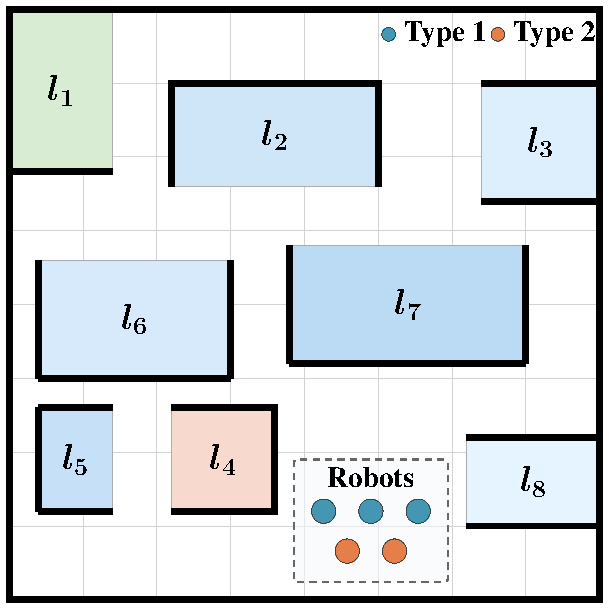
\includegraphics[width=2.0in]{pic/build/workspace_example1_editable.pdf}
\caption{Workspace of experiments.}
\label{workspace}
\end{figure}

\subsection{Problem Definition}
Consider an LTL formula \(\varphi\) over \(\mathcal{AP}\).
Let $B_\varphi=(Q_B,Q_{B,0},\Sigma_B,\rightarrow_B,Q_{B,F})$ be the NBA associated with \(\varphi\). Here, \(Q_B\) is the finite set of Buchi states, \(Q_{B,0}\) is the set of initial states, \(\Sigma_B=2^{AP}\) is the alphabet, \(\rightarrow_B\subseteq Q_B\times\Sigma_B\times Q_B\) is the transition relation, and \(Q_{B,F}\) is the set of accepting states.
 To connect the generated NBA structure with task-level planning, we associate each NBA transition with a subtask. 

\begin{definition}[Subtask]
Consider an NBA transition $(q_i,\sigma_{ij},q_j)\in\rightarrow_B$, where  \(q_i,q_j\in Q_B\) are NBA states. Let $\sigma_i^{\rm s}$ denote the self-loop condition at NBA state $q_i$.   If no holding condition is required, we set \(\sigma_i^{\rm s}=\top\). The subtask induced by this  transition is defined as below.
\begin{equation}
\omega_{ij}=(\sigma_{ij},\sigma_i^{\rm s}).
\end{equation}
Here, $\sigma_{ij}$ specifies the propositions that enable the transition from $q_i$ to $q_j$, while
$\sigma_i^{\rm s}$ specifies the propositions that must be maintained before this transition is
completed.
\end{definition}
% For a subtask \(\omega_{ij}\), let \(\mathcal A(\omega_{ij})\subseteq\mathcal A\) be the set of action propositions that appear as positive requirements in the transition label \(\sigma_{ij}\).
A plan of $\varphi$ is defined as $\Pi=(\boldsymbol{\omega}, \boldsymbol{\rho}, \boldsymbol{\mathcal C})$
where $ \boldsymbol{\omega}=\omega_0\omega_1\omega_2\cdots$ is the corresponding subtask sequence, $\boldsymbol{\rho}=q_0q_1q_2\cdots$ is the corresponding sequence of NBA states, $ \boldsymbol{\mathcal C}=\mathcal{C}_0\mathcal{C}_1\mathcal{C}_2\cdots$ is the corresponding robot-assignment sequence. Specifically,  for subtask $\omega_k$,  let $\mathcal A(\omega_k)\subseteq\mathcal A$ denote the set of action propositions that must be true at this transition. The assignment $ \mathcal{C}_k:\mathcal A(\omega_k)\rightarrow 2^{\mathcal R} $
maps each required action proposition to the set of robots selected to execute it. Assignments for different action propositions in the same $\omega_k$ must be disjoint, i.e., $ \mathcal{C}_k(a_i)\cap \mathcal{C}_k(a_j)=\emptyset,\qquad \forall a_i\neq a_j,\ a_i,a_j\in\mathcal A(\omega_k). $

The accepting run of NBA can be written in a prefix--suffix structure. Thus,  $\boldsymbol{\rho}$ can be 
written as $\boldsymbol{\rho}=\boldsymbol{\rho}_{\mathrm{pre}}\bigl(\boldsymbol{\rho}_{\mathrm{suf}}\bigr)^\omega$ , where $\boldsymbol{\rho}_{\mathrm{pre}}$ is the  prefix run and $\boldsymbol{\rho}_{\mathrm{suf}}$ is the suffix run. The corresponding plan $\Pi$ admits the same prefix--suffix structure, i.e. $\Pi = \Pi_{\mathrm{pre}}(\Pi_{\mathrm{suf}})^\omega$. Here, $ \Pi_{\mathrm{pre}}$ is the plan segment associated with $\boldsymbol{\rho}_{\mathrm{pre}}$ , and $\Pi_{\mathrm{suf}}$ is the finite plan segment associated with one traversal of the suffix cycle $\boldsymbol{\rho}_{\mathrm{suf}}$. To represent one completed execution of the prefix--suffix plan, we define the finite plan  \(\Pi_{\mathrm{fin}} =
\Pi_{\mathrm{pre}}\Pi_{\mathrm{suf}}\).
Let $T(\Pi_{\mathrm{fin}})$ denote the completion time of $\Pi_{\mathrm{fin}}$. The cost is defined as below.
\begin{equation} \label{objective}
J_\varphi=T(\Pi_{\mathrm{fin}}).
\end{equation}

\begin{problem}
Consider a  workspace $\mathcal{W}$ and a heterogeneous robot team $\mathcal{R}$ with type set $\mathcal{T}$, and a LTL formula $\varphi$ defined over the atomic proposition set $\mathcal{AP}=\mathcal{P} \cup \mathcal{A}$.  The goal is to develop a task plan for  each robot such that the specification $\varphi$ is satisfied and the cost in Eq. \ref{objective} is minimized.
\end{problem}

\section{System  Overview} \label{sec:system_overview}

% This section presents the proposed framework for LTL-MRTA. The key idea is to incorporate planning information into the LTL-to-automaton translation process, rather than constructing the complete NBA before planning. Following the LTL2BA pipeline, the LTL formula is first transformed into an abstract syntax tree, then into a very weak alternating automaton (VWAA), and subsequently into a generalized B"uchi automaton (GBA). During the VWAA-to-GBA construction, candidate transitions that cannot be satisfied by the available robot team are pruned immediately. After the GBA is generated, decomposition-inducing transitions are further removed to avoid unnecessary synchronization among independent subtasks.

% Based on the pruned GBA, the NBA and a shared directed plan graph are constructed synchronously. Each generated NBA transition induces a subtask, which is evaluated on the fly using the predicted robot positions and completion times stored in the plan graph. In this way, infeasible branches are discarded early, while feasible task progressions are incrementally recorded in the plan graph. Once an accepting prefix--suffix structure is reached, an initial feasible plan is extracted from the graph and then further optimized by a warm-started branch-and-bound procedure.
This section presents the proposed framework for LTL-MRTA, as summarized in Algorithm~\ref{alg:framework}. The key idea is to integrate task-allocation reasoning into the LTL-to-automaton translation process, instead of constructing the complete NBA before planning. Specifically, the input LTL formula is first parsed into an abstract syntax tree and then translated into a VWAA following the LTL2BA pipeline. During the subsequent GBA construction, transitions that cannot be realized by the available robot team are pruned immediately. After the GBA is generated, decomposition-inducing transitions are further removed to avoid unnecessary synchronization among independent subtasks.

Given the pruned GBA, the framework constructs the NBA and a shared directed plan graph synchronously. Each newly generated NBA transition induces a subtask, which is evaluated on the fly using the robot assignments, predicted positions, and completion times stored in the current plan node. Infeasible successors are discarded, whereas feasible task progressions are inserted into the plan graph. Once an accepting prefix--suffix structure is reached, an initial feasible plan is extracted. After the plan graph is completed, this feasible plan is used to warm-start a branch-and-bound optimizer, which further improves the completion time over the generated plan graph.



\begin{algorithm}[H]
\caption{On-the-fly Task Allocation framework} \label{alg:framework}
\begin{algorithmic}[1]
\REQUIRE LTL formula $\varphi$, workspace $\mathcal{W}$, robot team $\mathcal{R}$, atomic propositions $\mathcal{AP}$.
\ENSURE Feasible plan $\Pi^\star$.
\STATE Parse $\varphi$ and construct the VWAA $\mathcal{V}_\varphi$.
\STATE Construct and prune the GBA $\mathcal{G}^{-}_\varphi$.
\STATE Initialize the root plan node $\nu_0$.
\STATE $(G_P,\Pi_{\rm init})\gets
\textsc{ConstructPlanGraph}(\mathcal{G}^{-}_\varphi,\mathcal R,\nu_0)$.
\STATE $\Pi^\star\gets$ \text{BnB\_Optimizer}($G_P,\Pi_{\rm init}$).
\RETURN $\Pi^\star$.
\end{algorithmic}
\end{algorithm}

 \section{Pruning for GBA} 

In this section, we introduce the proposed pruning procedure during the construction of GBA. Unlike methods that perform pruning  after the complete NBA has been constructed, the proposed method prunes the GBA both
during and after the VWAA-to-GBA construction stage. This early pruning reduces the size of the GBA and  prevents unnecessary transitions from being propagated to the subsequent NBA construction and planning stages. The proposed GBA pruning consists of the following two parts. 

\subsubsection{Infeasible Transition Pruning During GBA Construction}  \label{subsec:infeasible_gba_pruning}

The simplifications performed during the construction of  GBA rely  on the logical formula and the evolving automaton structure, without incorporating information about the robot team or the workspace. We therefore introduce a robot-team feasibility check during GBA construction.
Before a candidate transition $ e_g=(q_g,\sigma_g,q_g')$
is inserted into \(\rightarrow_g\), the action requirements in
\(\sigma_g\) are checked against the available robot team \(\mathcal{R}\). If no subset of \(\mathcal{R}\) can satisfy the 
requirements, \(e_g\) is infeasible for the considered system and is discarded immediately. Otherwise, it is retained for subsequent GBA construction.
For example, suppose that a candidate transition requires three type-1 robots to perform an action at region \(l_1\) and another three type-1 robots to perform an action at region \(l_2\) simultaneously. If $\mathcal{R}$ contains only five type-1 robots, no feasible robot assignment can satisfy the transition condition. The candidate
transition is therefore discarded before it is inserted into $\rightarrow_g$.


% In the VWAA-to-GBA construction,  a GBA state \(q_g\in Q_g\) corresponds to a conjunction of VWAA states, i.e. represents a set of VWAA states that must hold simultaneously. Suppose that
% $ q_g = q_{v,1}\wedge q_{v,2}\wedge \cdots \wedge q_{v,n}, $
% where \(q_{v,i}\in Q_v\). For each VWAA state \(q_{v,i}\), its transition \(\delta_v(q_{v,i})\) provides possible ways
% to move from \(q_{v,i}\) to a set of successor VWAA states under input conditions. To construct an outgoing GBA transition from \(q_g\), one transition is selected from each \(\delta_v(q_{v,i})\), and these selected VWAA transitions are combined. Their input conditions are conjoined, and their successor VWAA states are collected to form the successor GBA state \(q_g'\in Q_g\). Thus, each such combination produces a  GBA transition
% $ q_g \xrightarrow{\sigma} q_g', $
% where \(\sigma\in\Sigma\) denotes the input symbol satisfying the combined transition condition.
% The accepting structure is also transferred during this construction. The co-B\"uchi accepting states \(F_v\) of the VWAA are transformed into the collection of accepting transition sets \(F_g=\{F_{g,1},\ldots,F_{g,m}\}\) of the GBA. Therefore, GBA acceptance is checked on transitions rather than on states: a run of \(G_\varphi\) is accepting if it traverses transitions in every accepting transition set in \(F_g\) infinitely often.

% Building on the above construction, we further introduce infeasible transition pruning during GBA generation to eliminate transitions that cannot be realized by the considered multi-robot system. Specifically, for a GBA transition, if no robot combination in $\mathcal{R}$ can satisfy its transition condition, then this transition is called an infeasible transition. For example, suppose that a transition requires three type-1 robots to execute an action at region \(l_1\) and, at the same time, another three type-1 robots to execute an action at region \(l_2\). If the robot
% team $\mathcal{R}$ contains only five type-1 robots in total, then no robot combination can satisfy this transition condition. Therefore, this transition is infeasible and can be removed during GBA construction. 
% During the construction, infeasible transition pruning is performed when outgoing GBA transitions are being generated. For a GBA state \(q_g\), the outgoing transitions are obtained by combining the outgoing transitions of the VWAA
% states.  Before this  transition is inserted into \(\rightarrow_g\), we check whether its transition condition can be satisfied by the  robot team \(\mathcal{R}\). If no robot combination in \(\mathcal{R}\) can satisfy the condition, the candidate transition is identified as infeasible and is discarded immediately. Otherwise, the transition is kept, and the  GBA construction continues.

\subsubsection{Pruning of Progress-Consistent Decomposable Transitions}
The second pruning step is performed after the GBA has been constructed. Although pruning is applied at the GBA level, it targets unnecessary synchronization that would otherwise be inherited by the resulting NBA. Since each NBA transition induces a subtask, requiring several independent subtasks to be satisfied at the same transition  can be unnecessarily restrictive \cite{liu2024time}. The main challenge is to identify and remove such synchronization before the
complete NBA is available. A GBA transition can therefore be removed only when decomposing its combined task requirements preserves the
acceptance progress used in the subsequent GBA-to-NBA degeneralization. To formalize this decomposition without restricting it to a particular
automaton type, we first introduce a general definition of transition decomposability. The definition applies to both NBA and GBA
transitions.

\begin{definition}[Decomposable transition]
\label{def:decomposable_transition}
Consider an automaton with state set $Q$, alphabet $\Sigma$, and transition relation $\rightarrow\subseteq Q\times\Sigma\times Q$.
A transition $e_{ij}=(q_i,\sigma_{ij},q_j)\in\rightarrow$ is called decomposable if there exist a state $q_k\in Q$ and two
transitions $(q_i,\sigma_{ik},q_k)\in\rightarrow$ and $(q_k,\sigma_{kj},q_j)\in\rightarrow$ such that
$\sigma_{ij}=\sigma_{ik}\cup\sigma_{kj}$.
\end{definition}

Definition~\ref{def:decomposable_transition} applies to both NBA and GBA transitions. For GBA pruning, however, decomposability alone is not sufficient because degeneralization also tracks progress through multiple accepting transition sets. We therefore call a decomposable GBA transition progress-consistent if its decomposition produces the same acceptance-progress update as the original transition for every degeneralization index. Only progress-consistent decomposable transitions are eligible for pruning.
Let $m_g:=|\mathcal{F}_g|$ and
$\mathcal{F}_g=\{F_{g,1},\ldots,F_{g,m_g}\}$. For a GBA transition $e^g\in\rightarrow_g$, define its acceptance-set index set as
$\operatorname{Acc}(e^g):=
\{h\in\{1,\ldots,m_g\}\mid e^g\in F_{g,h}\}$.
Each state of the degeneralized NBA is represented by $(q_g,\ell)$, where $\ell\in\mathcal{I}_F:=\{0,\ldots,m_g\}$ is the current acceptance-progress index. Let $\eta(\ell,e^g)$ denote the progress
obtained after traversing $e^g$ from progress $\ell$. Set $\bar{\ell}=0$ if $\ell=m_g$ and $\bar{\ell}=\ell$ otherwise. Then $\eta(\ell,e^g):=
\max\{r\in\{\bar{\ell},\ldots,m_g\}\mid
\{\bar{\ell}+1,\ldots,r\}\subseteq
\operatorname{Acc}(e^g)\}$.
This update provides a direct test of progress consistency. Given an initial progress $\ell$, the candidate decomposition first computes $\eta(\ell,e^g_{ik})$ and passes the returned index to $e^g_{kj}$ to obtain $\eta(\eta(\ell,e^g_{ik}),e^g_{kj})$. This result is compared with $\eta(\ell,e^g_{ij})$, and the decomposition is accepted when the two updates agree for all admissible initial progress indices. The following definition formalizes this criterion.
 
\begin{definition}[Progress-consistent decomposable transition]
\label{def:progress_consistent_decomposable_transition}
A decomposable GBA transition $e^g_{ij}\in\rightarrow_g$ is called progress-consistent decomposable if it admits a decomposition 
$(e^g_{ik},e^g_{kj})$ according to
Definition~\ref{def:decomposable_transition} such that
$\eta(\eta(\ell,e^g_{ik}),e^g_{kj})
=\eta(\ell,e^g_{ij})$ for every
$\ell\in\mathcal{I}_F$. Such a pair
$(e^g_{ik},e^g_{kj})$ is called a progress-consistent decomposition
witness of $e^g_{ij}$.
\end{definition}


\begin{lemma}\label{l1}
Every NBA transition induced by a progress-consistent decomposable GBA transition is decomposable.
\end{lemma}

\begin{proof} \label{l2}
Let $e^g_{ij}=(q_{g,i},\sigma_{ij},q_{g,j})$ be a
progress-consistent decomposable GBA transition, and let
$(e^g_{ik},e^g_{kj})$ be one of its progress-consistent decomposition transitions, where
$e^g_{ik}=(q_{g,i},\sigma_{ik},q_{g,k})$ and
$e^g_{kj}=(q_{g,k},\sigma_{kj},q_{g,j})$.
Fix an arbitrary acceptance-progress index $\ell\in\mathcal{I}_F$. The transition $e^g_{ij}$ induces the NBA transition
$((q_{g,i},\ell),\sigma_{ij},
(q_{g,j},\eta(\ell,e^g_{ij})))$.
The transition induces successive NBA transitions through
$(q_{g,k},\eta(\ell,e^g_{ik}))$, with terminal state
$(q_{g,j},\eta(\eta(\ell,e^g_{ik}),e^g_{kj}))$.
By progress consistency,
$\eta(\eta(\ell,e^g_{ik}),e^g_{kj})
=\eta(\ell,e^g_{ij})$. Thus, both representations reach the same terminal NBA state. Moreover,
$\sigma_{ij}=\sigma_{ik}\cup\sigma_{kj}$ follows from
Definition~\ref{def:decomposable_transition}. Therefore, the NBA transition induced by $e^g_{ij}$ is decomposable. Since $\ell$ is arbitrary, the result holds for every NBA transition induced by $e^g_{ij}$.
\end{proof}

\begin{lemma}\label{l3}
If a feasible solution can be generated from the original GBA, then an equivalent feasible solution can also be generated from the pruned GBA.
\end{lemma}
\begin{proof}
Let $\mathcal{B}_{\varphi}$ and $\mathcal{B}_{\varphi}^{-}$ be the NBAs generated from the original and pruned GBAs, respectively. Consider a feasible solution $\Pi$ represented by an accepting run $\rho$ of $\mathcal{B}_{\varphi}$.
A GBA transition removed by infeasible-transition pruning cannot
induce a transition used by $\Pi$. Otherwise, $\Pi$ would contain a task requirement that cannot be satisfied by the robot team, which contradicts its feasibility.
Now consider a progress-consistent decomposable GBA transition
removed during the second pruning step. By Lemma~\ref{l1}, every NBA
transition induced by this GBA transition is decomposable. The
corresponding decomposition reaches the same terminal NBA state and
preserves the acceptance progress. Moreover, its transition labels
jointly reproduce the original transition label. Thus, the
decomposition introduces no additional task requirements.
Applying the decomposition to every affected transition in $\rho$
produces an accepting run of $\mathcal{B}_{\varphi}^{-}$. If a
transition involved in a decomposition is also pruned, its own
decomposition is applied in the pruning order. Since the GBA contains
finitely many transitions, this decomposition process terminates with
transitions retained in the pruned GBA. The resulting accepting run
represents a feasible solution equivalent to $\Pi$.
\end{proof}

\section{On-the-Fly Plan Graph Construction}
\label{subsec:plan_graph_construction}

After GBA-level pruning, the NBA and the plan graph are constructed synchronously. As the NBA is generated, each candidate transition induces a subtask. The greedy allocation procedure evaluates this subtask from the current plan nodes. A successful allocation extends the plan graph and updates the predicted execution state of the robot team. Once an accepting prefix--suffix structure is reached, an executable plan can be extracted without constructing the complete NBA.
To guide this joint construction, a residual-obligation score is used to order newly generated NBA states. In contrast to the original LTL2BA construction, which follows the DFS generation order, the proposed method gives priority to states associated with more promising partial plans. Since the plan graph grows together with the NBA, this ordering also guides the exploration of task-allocation branches and helps obtain a high-quality initial plan earlier.

% Let
% \(G_\varphi=(Q_g,Q_{g,0},\Sigma,\rightarrow_g,F_g)\) be the pruned GBA with \(F_g=\{F_{g,1},\ldots,F_{g,m}\}\). Each NBA state is represented as \(q_B=(q_g,\ell)\), where \(q_g\in Q_g\) is a GBA state and \(\ell\in\{0,1,\ldots,m\}\) records the current progress through the accepting transition sets. Whenever a new NBA transition
% is generated, the induced subtask is immediately evaluated at the planning level.

\subsection{Plan Graph and Plan Node}
During NBA construction, feasible  task allocations are
incrementally recorded in a plan graph. Each plan node associates an NBA state with the corresponding robot assignment and predicted execution state.  A plan node is formally defined as follows.
\begin{definition}[Plan node]\label{def:plan_node}
Consider the plan graph $G_P=(V_P,E_P),$ where \(V_P\) is the set of plan nodes and \(E_P\subseteq V_P\times V_P\) is the set of directed edges.
Each plan node is denoted by \(\nu_i\), and $V_P=\{\nu_i\mid i=0,1,\ldots,N_P\},$
where \(\nu_0\) is the root node and \(N_P+1\) is the number of nodes in the generated plan graph. Each plan node \(\nu_i\in V_P\) is defined as
\[
\nu_i =
(q_{B,i},\mathrm{Prog}_i,\omega_i,\mathcal{C}_i,X_i,\Theta_i).
\]
Here, \(q_{B,i}\in Q_B\) is the NBA state associated with \(\nu_i\), and
\(\mathrm{Prog}_i\in\{\mathrm{pre},\mathrm{suf},\mathrm{acc},\mathrm{dead}\}\)
denotes the planning status of \(\nu_i\). Specifically,
\(\mathrm{Prog}_i=\mathrm{pre}\) indicates that the current node is in the prefix stage and 
\(\mathrm{Prog}_i=\mathrm{suf}\) indicates that the current node is in the suffix stage. 
\(\mathrm{Prog}_i=\mathrm{acc}\) indicates that the node completes an accepting prefix--suffix structure, while \(\mathrm{Prog}_i=\mathrm{dead}\) indicates that
the candidate is discarded and will not be further expanded. For each
non-root node \(\nu_i\), \(\operatorname{par}(\nu_i)\) denotes the predecessor
used to compute its stored execution state and to extract the plan.
\(\omega_i\) is the subtask associated with \(\nu_i\), and \(\mathcal{C}_i\) is the
corresponding robot assignment.
The vector
$X_i=(x_i(r_1),x_i(r_2),\ldots,x_i(r_{n_r}))$ denotes the predicted
robot positions, where \(x_i(r_k)\) is the predicted position of robot
\(r_k\) at plan node \(\nu_i\). The vector
$\Theta_i=(\theta_i(r_1),\theta_i(r_2),\ldots,\theta_i(r_{n_r}))$
denotes the predicted completion times, where \(\theta_i(r_k)\) is the
predicted completion time of robot \(r_k\).
\end{definition}

By Definition~\ref{def:plan_node}, a plan node records the progress in the automaton and the predicted execution state of the robot team. Specifically, \(q_{B,i}\), \(\mathrm{Prog}_i\), and \(\omega_i\)
describe where the current partial plan is in the NBA and which subtask is being considered. The assignment \(\mathcal{C}_i\) specifies which robots execute the current subtask, while \(X_i\) and \(\Theta_i\) summarize the predicted robot configuration after this subtask is completed.
%在这里补充上例子的具体数据（tree是多少，graph是多少）
\subsection{Construction of Plan Graph}  %需要按照前缀后缀进行修改，特别是lower bound那部分
%可以增加一个整体概述
The plan graph is constructed synchronously with the NBA. The root
node is initialized as
\(\nu_0=(q_{B,0},\mathrm{pre},\emptyset,\emptyset,X_0,\Theta_0)\).
For each robot \(r_k\in\mathcal R\), its initial predicted position
and completion time are \(x_0(r_k)=x(r_k)\) and
\(\theta_0(r_k)=0\), respectively. The same NBA state may be reached through different task-allocation sequences. These sequences may result in different robot assignments and predicted execution states. Therefore, multiple plan nodes may be associated with the same NBA state. For any plan node \(\nu_i\), its current plan cost is defined as follows.
\begin{equation}
J(\nu_i)
=
\max_{r_k\in\mathcal R}\theta_i(r_k).
\label{eq:plan-node-cost}
\end{equation}
When multiple plan nodes are associated with the same NBA state,
they are processed in nondecreasing order of this cost.

During construction, \(\mathcal S_B\) stores the NBA states waiting to be expanded, while \(Q_B^{\rm exp}\) contains the states that have already been expanded. For each state removed from \(\mathcal S_B\), the temporary set \(\mathcal P_B\) stores the newly discovered successor NBA states.
For each feasible extension from a parent plan node \(\nu_i\) along a
candidate transition \(e_{B,ij}\), the ordering score
\(S(\nu_i,e_{B,ij})\) is computed. A lower score gives the
corresponding successor NBA state higher priority. If several feasible
extensions reach the same successor state \(q_{B,j}\),
\(s_B(q_{B,j})\) retains their smallest score. The score computation
is presented in the residual-obligation scoring subsection.

\begin{algorithm}[t]
\caption{\textsc{ConstructPlanGraph}}
\label{alg:otf_pg}
\begin{algorithmic}[1]
\REQUIRE Pruned GBA $\mathcal{G}^{-}_\varphi$, robot team $\mathcal R$,
and initial plan node $\nu_0$.
\ENSURE Plan graph $G_P$ and initial plan $\Pi_{\rm init}$.

\STATE $G_P\gets(\{\nu_0\},\emptyset)$.
\STATE $\mathcal S_B\gets[q_{B,0}]$ and
$Q_B^{\rm exp}\gets\emptyset$.
\STATE $\Pi_{\rm init}\gets\emptyset$.

\WHILE{$\mathcal{S}_B\neq\emptyset$}
    \STATE $q_{B,i}\gets\operatorname{Pop}(\mathcal S_B)$.
    \STATE $Q_B^{\rm exp}\gets Q_B^{\rm exp}\cup\{q_{B,i}\}$.
    \STATE $\mathcal P_B\gets\emptyset$.
    \STATE Generate the candidate NBA transitions from $q_{B,i}$.
    \STATE Simplify the candidate transitions from $q_{B,i}$ using the
    on-the-fly transition rule of LTL2BA.

    \FORALL{remaining candidate transition
    $e_{B,ij}:q_{B,i}\xrightarrow{\sigma_{ij}}q_{B,j}$}
        \FORALL{plan node $\nu_i$ associated with $q_{B,i}$, in
        nondecreasing order of $J(\nu_i)$}
            \STATE $\nu_j\gets
            \textsc{ExtendPlanGraph}(G_P,\nu_i,e_{B,ij},\mathcal R)$.

            \IF{$\nu_j\neq\emptyset$}
                \IF{$\nu_j.\mathrm{Prog}=\mathrm{acc}$}
                    \IF{$\Pi_{\rm init}=\emptyset\lor
                    J(\nu_j)<T(\Pi_{\rm init})$}
                        \STATE Set \(\Pi_{\rm init}\) to the plan extracted
                        from \(\nu_j\).
                    \ENDIF
                \ELSE
                    \STATE Update $\mathcal M_j$ using the remaining sets
                    of the parent nodes of $\nu_j$.
                    \STATE Compute $S(\nu_i,e_{B,ij})$ according to
                    Eq.~\ref{eq:score}.
                    \IF{$q_{B,j}\in Q_B^{\rm exp}$}
                        \STATE \textsc{ReuseSuccessors}$(G_P,\nu_j,\mathcal R)$.
                    \ELSIF{$q_{B,j}\notin\mathcal S_B$}
                        \IF{$q_{B,j}\notin\mathcal P_B$}
                            \STATE $\mathcal P_B\gets
                            \mathcal P_B\cup\{q_{B,j}\}$.
                            \STATE $s_B(q_{B,j})\gets
                            S(\nu_i,e_{B,ij})$.
                        \ELSE
                            \STATE $s_B(q_{B,j})\gets
                            \min\{s_B(q_{B,j}),S(\nu_i,e_{B,ij})\}$.
                        \ENDIF
                    \ENDIF
                \ENDIF
            \ENDIF
        \ENDFOR
    \ENDFOR

    \STATE Sort the states in $\mathcal P_B$ by nondecreasing
    $s_B$, using generation order to break ties.
    \STATE Push them onto $\mathcal S_B$ in reverse order.
\ENDWHILE

\STATE Apply the simplification in
Section~\ref{subsec:final_pruning} to \(G_P\).
\RETURN $(G_P,\Pi_{\rm init})$.
\end{algorithmic}
\end{algorithm}

Algorithm~\ref{alg:otf_pg} summarizes the overall construction
procedure. When an NBA state \(q_{B,i}\) is expanded, its candidate
outgoing transitions are generated. Before planning, these transitions
are simplified using the on-the-fly rule of LTL2BA
\cite{Gastin2001FastLT}. On-the-fly automaton simplification is one of
the main improvements of LTL2BA. Each new transition is compared with
the transitions already generated from the same NBA state. If two
transitions have the same successor and the condition of one implies that of the other, the former is removed immediately. For each remaining transition
\(e_{B,ij}:q_{B,i}\xrightarrow{\sigma_{ij}}q_{B,j}\), the plan nodes associated with \(q_{B,i}\) are processed in nondecreasing order of their costs. For each parent--transition pair, \textsc{ExtendPlanGraph} first attempts to generate a feasible successor plan node. An accepting successor terminates its branch and provides a candidate plan. For every other feasible successor, its remaining set is updated and its ordering score is computed according to Eq.~\ref{eq:score}. A feasible
successor state that has neither been expanded nor placed in \(\mathcal S_B\) is added to \(\mathcal P_B\). If several feasible extensions reach the same successor state, only the smallest score is
retained. The states in \(\mathcal P_B\) are then ordered by their retained scores and added to \(\mathcal S_B\).

% when a newly generated plan node \(\nu_j\) is associated with an NBA state \(q_{B,j}\) 

% that has already been expanded, the outgoing NBA transitions of \(q_{B,j}\) are not generated again. Instead, \(\nu_j\) is connected to each existing successor plan node \(\nu_h\)
% generated from the same NBA state and progress flag. If \(J(\nu_j)\) is smaller than the costs of all other parent nodes of \(\nu_h\), then \(\nu_j\) becomes its representative predecessor. The robot assignment
% and predicted execution state of \(\nu_h\) are recomputed from \(\nu_j\), and the update is propagated to its descendants. Otherwise, only the new edge is retained, and the stored execution state of \(\nu_h\) remains unchanged.

Whenever a returned plan node \(\nu_j\) satisfies
\(\nu_j.\mathrm{Prog}=\mathrm{acc}\), its plan is extracted. The
extracted plan replaces \(\Pi_{\rm init}\) only if
\(\Pi_{\rm init}\) is empty or \(J(\nu_j)<T(\Pi_{\rm init})\).
Therefore, \(\Pi_{\rm init}\) stores the lowest-cost accepting plan
found during construction. After all pending NBA states have been
processed, the plan graph is simplified according to
Section~\ref{subsec:final_pruning}. The algorithm then returns the
simplified plan graph \(G_P\) and \(\Pi_{\rm init}\).
The \textsc{ExtendPlanGraph} procedure is presented in
Algorithm~\ref{alg:extend_successor}.

\begin{algorithm}[H]
\caption{\textsc{ExtendPlanGraph}}
\label{alg:extend_successor}
\begin{algorithmic}[1]
\REQUIRE Plan graph $G_P$, parent node $\nu_i$, NBA transition
$e_{B,ij}:q_{B,i}\xrightarrow{\sigma_{ij}}q_{B,j}$, and robot team $\mathcal R$.
\ENSURE Successor plan node $\nu_j$, or $\emptyset$ if the assignment fails.
\STATE Obtain the induced subtask
$\omega_{ij}=(\sigma_{ij},\sigma_i^{\mathrm{s}})$.
\STATE Compute the successor progress flag $\mathrm{Prog}_j$, setting
$\mathrm{Prog}_j\gets\mathrm{acc}$ if the extension completes an
accepting prefix--suffix structure.
\STATE $\nu_h\gets$ a plan node associated with $q_{B,j}$ whose progress flag is $\mathrm{Prog}_j$ and whose subtask is $\omega_{ij}$, if one exists.
\STATE $(\hat{\mathcal C},\hat{X},\hat{\Theta},\hat{J})\gets
\textsc{GreedyAssign}(\omega_{ij},\nu_i,\mathcal R)$.
\IF{\textsc{GreedyAssign} fails}
    \RETURN $\emptyset$.
\ENDIF
\IF{$\nu_h$ exists}
    \STATE Add $(\nu_i,\nu_h)$ to $E_P$.
    \IF{$\hat{J}<J(\nu_h)$}
        \STATE Set $\operatorname{par}(\nu_h)\gets\nu_i$, $\mathcal C_h\gets\hat{\mathcal C}$, $X_h\gets\hat{X}$, and $\Theta_h\gets\hat{\Theta}$; propagate the improvement to descendants.
    \ENDIF
    \STATE $\nu_j\gets\nu_h$.
\ELSE
    \STATE Create $\nu_j=(q_{B,j},\mathrm{Prog}_j,\omega_{ij},\hat{\mathcal C},\hat{X},\hat{\Theta})$.
    \STATE Set $\operatorname{par}(\nu_j)\gets\nu_i$, insert $\nu_j$ into $V_P$, and add $(\nu_i,\nu_j)$ to $E_P$.
\ENDIF
\IF{$\nu_j.\mathrm{Prog}=\mathrm{acc}$}
    \STATE Record $\nu_j$ as a feasible solution leaf.
\ENDIF
\RETURN $\nu_j$.
\end{algorithmic}
\end{algorithm}
\subsubsection{ExtendPlanGraph} \label{gen}

Algorithm~\ref{alg:extend_successor} extends the plan graph from a parent plan node \(\nu_i\) along an NBA transition
\(e_{B,ij}\).
It first constructs the induced subtask
\(\omega_{ij}=(\sigma_{ij},\sigma_i^{\mathrm{s}})\) and computes the
successor progress flag \(\mathrm{Prog}_j\). The flag records whether
the extension remains in the prefix stage, enters the suffix stage, or
completes an accepting prefix--suffix structure.
An existing plan node \(\nu_h\) is compatible with this extension if it is associated with \(q_{B,j}\) and satisfies
\(\mathrm{Prog}_h=\mathrm{Prog}_j\) and \(\omega_h=\omega_{ij}\).

The procedure next calls function \textsc{GreedyAssign}\((\omega_{ij},\nu_i,\mathcal R)\) to evaluate the candidate extension. For each required action proposition \(a_\ell\in\mathcal A(\omega_{ij})\), the execution requirement \(c(a_\ell)=(\tau_\ell,n_\ell,l_\ell)\) specifies the required robot
type, number of robots, and target region. For every robot
\(r_k\in\mathcal R_{\tau_\ell}\), its predicted arrival time from
\(\nu_i\) is computed as follows.
\begin{equation}
\hat t_i(r_k,a_\ell)
=
\theta_i(r_k)
+
\frac{d_k(x_i(r_k),l_\ell)}{v(r_k)}.
\label{eq:predicted_arrival}
\end{equation}
Here, \(x_i(r_k)\) and \(\theta_i(r_k)\) are stored in \(\nu_i\).
A robot is eligible for \(a_\ell\) if its predicted arrival time is
finite and it has not been assigned to another action proposition in
the same subtask.

The action propositions in \(\mathcal A(\omega_{ij})\) are processed
in increasing order of their indices. For each \(a_\ell\), the
\(n_\ell\) eligible robots with the smallest predicted arrival times
are selected and stored in \(\hat{\mathcal C}(a_\ell)\). The predicted
positions of the selected robots are updated to the corresponding
target regions, and their predicted completion times are set to the
latest predicted arrival time among all robots assigned to
\(\omega_{ij}\). Robots not assigned to \(\omega_{ij}\) retain their
states from \(X_i\) and \(\Theta_i\).

These updates produce
\(\hat X=(\hat x(r_1),\ldots,\hat x(r_{n_r}))\) and
\(\hat\Theta=(\hat\theta(r_1),\ldots,\hat\theta(r_{n_r}))\).
The resulting node cost is
\(\hat J=\max_{r_k\in\mathcal R}\hat\theta(r_k)\).
If fewer than \(n_\ell\) eligible robots are available for any required
action proposition, \textsc{GreedyAssign} fails and the candidate
extension is discarded.

If \textsc{GreedyAssign} succeeds and a compatible plan node
\(\nu_h\) exists, \textsc{ExtendPlanGraph} adds
\((\nu_i,\nu_h)\) to \(E_P\). If \(\hat J<J(\nu_h)\), the representative predecessor of \(\nu_h\) is updated to \(\nu_i\). Its robot assignment, predicted positions, and predicted completion times are replaced by
\(\hat{\mathcal C}\), \(\hat X\), and \(\hat\Theta\), respectively. The resulting improvement is then propagated to its successor nodes. If no compatible plan node exists, a new node
\(\nu_j=(q_{B,j},\mathrm{Prog}_j,\omega_{ij},
\hat{\mathcal C},\hat X,\hat\Theta)\) is created.
Its representative predecessor is set to \(\nu_i\). The new node is inserted into \(V_P\), and the edge \((\nu_i,\nu_j)\) is added to \(E_P\).


\subsubsection{Reuse of Existing Successors}

When a plan node \(\nu_j\) reaches an NBA state \(q_{B,j}\) that has
already been expanded, its outgoing NBA transitions and successor
structure are already available. Therefore, these transitions are not
generated again. The \textsc{ReuseSuccessors} procedure connects
\(\nu_j\) to the existing successor plan nodes and determines whether
their representative execution states should be updated.

\begin{algorithm}[H]
\caption{\textsc{ReuseSuccessors}}
\label{alg:reuse_successors}
\begin{algorithmic}[1]
\REQUIRE Plan graph \(G_P\), plan node \(\nu_j\) associated with
\(q_{B,j}\in Q_B^{\rm exp}\), and robot team \(\mathcal R\).
\ENSURE Updated plan graph \(G_P\).

\FORALL{$(\nu_p,\nu_h)\in E_P:
q_{B,p}=q_{B,j},\
\mathrm{Prog}_p=\mathrm{Prog}_j,\
(\nu_j,\nu_h)\notin E_P$}
    \STATE Add \((\nu_j,\nu_h)\) to \(E_P\).
    \IF{$J(\nu_j)<
    \min\{J(\nu_\ell)\mid
    (\nu_\ell,\nu_h)\in E_P,\
    \nu_\ell\neq\nu_j\}$}
        \STATE Set \(\operatorname{par}(\nu_h)\gets\nu_j\).
        \STATE Recompute \(\mathcal C_h\), \(X_h\), and
        \(\Theta_h\) from \(\nu_j\).
        \STATE Propagate the update to the descendants of \(\nu_h\).
    \ENDIF
\ENDFOR
\end{algorithmic}
\end{algorithm}

For each existing successor \(\nu_h\), the new edge is retained. If
\(\nu_j\) has the smallest cost among the parent nodes of \(\nu_h\),
it is selected as the representative predecessor. The robot
assignment and predicted execution state of \(\nu_h\) are then
recomputed from \(\nu_j\). Its cost is updated accordingly, and the
updated state is propagated to its descendants. Otherwise, the
representative predecessor and the stored execution state of
\(\nu_h\) remain unchanged.
This cost-based update follows the planning-decision-tree rule of
Chen et al.~\cite{Chen2024RealTimeReactive}, which was validated
experimentally.



%补充伪代码、例子
\subsubsection{Residual-Obligation Scoring of NBA States}

After a feasible nonaccepting successor plan node has been generated,
Algorithm~\ref{alg:otf_pg} updates its remaining set and computes the
ordering score \(S(\nu_i,e_{B,ij})\). The score is used to order the
successor NBA state \(q_{B,j}\) in the current pending set
\(\mathcal P_B\). It combines the current plan cost
\(J(\nu_i)\) with an estimate of the positive action requirements that
remain.

This estimate is based on a must-eventually action set extracted once
from the abstract syntax tree \(\mathcal T_\varphi\). For each
subformula \(\psi\), \(\mathsf{ME}(\psi)\subseteq\mathcal A\) denotes
a set of positive action propositions that must each be executed at
least once during the subsequent execution for \(\psi\) to be
satisfied. This set is obtained using the recursive rules below. The
remaining set associated with each plan node \(\nu_i\) is denoted by
\(\mathcal M_i\). At the root node \(\nu_0\), it is initialized as
\(\mathcal M_0=\mathsf{ME}(\varphi)\). In AST,
\(\lozenge\psi\) and \(\square\psi\) are represented in
\(\mathcal T_\varphi\) as \(\top\,\mathcal U\,\psi\) and
\(\bot\,\mathcal V\,\psi\), respectively.
\begin{enumerate}
 \item  The constants \(\top\) and \(\bot\) do not introduce any positive action proposition that must be completed. That is, if \(\psi=\top\) or \(\psi=\bot\), then $\mathsf{ME}(\psi)=\emptyset .$
 \item If \(\psi=a\) with \(a\in\mathcal A\), then
 \(\mathsf{ME}(\psi)=\{a\}\). If \(\psi=p\) with
 \(p\in\mathcal P\), or if \(\psi=\neg\pi\) with
 \(\pi\in\mathcal{AP}\), then
 \(\mathsf{ME}(\psi)=\emptyset\). That is, only positive action
 propositions are included.
  \item If \(\psi=\psi_1\wedge\psi_2\), then $  \mathsf{ME}(\psi)=\mathsf{ME}(\psi_1)\cup \mathsf{ME}(\psi_2).$
    Since both subformulas must be satisfied, the action propositions are collected from both sides.
  \item If \(\psi=\psi_1\vee\psi_2\), then $  \mathsf{ME}(\psi)= \mathsf{ME}(\psi_1)\cap \mathsf{ME}(\psi_2). $
    Since either branch may be selected, only action propositions that are unavoidable in both branches are kept.
  \item If \(\psi=\bigcirc\psi_1\), then $\mathsf{ME}(\psi)=\mathsf{ME}(\psi_1). $ The next operator shifts the satisfaction time but does not change the unavoidable positive action propositions.
  \item If
  \(\psi=\psi_1\,\mathcal U\,\psi_2\) or
  \(\psi=\psi_1\,\mathcal V\,\psi_2\), then
  \(\mathsf{ME}(\psi)=\mathsf{ME}(\psi_2)\), where
  \(\mathcal V\) denotes the release operator. In both cases, the
  positive action propositions retained from the right operand must be
  satisfied during the subsequent execution.
\end{enumerate}

The set \(\mathcal M_i\) is a formula-level summary of unavoidable positive action propositions rather than a set that must be satisfied immediately at the node $\nu_i$. It is used to estimate the remaining
effort before all future subtasks have been generated.

For a feasible successor plan node \(\nu_j\), its remaining set
combines those of its parent nodes and then removes the positive action
propositions executed by the induced subtask. It is updated as follows.
\begin{equation}
\mathcal M_j
=
\left(
\bigcup_{(\nu_i,\nu_j)\in E_P}\mathcal M_i
\right)
\setminus
\mathcal A(\omega_{ij}).
\end{equation}
For each $a\in\mathcal M_j$ with $c(a)=(\tau_a,n_a,l_a)$, we compute the arrival-time
estimates of all robots in $\mathcal R_{\tau_a}$ using the predicted positions $X_i$ and completion
times $\Theta_i$ stored in $\nu_i$, and take the $n_a$-th
smallest value, denoted by $h_a(\nu_i)$. The residual pressure of $(\nu_i,e_{B,ij})$ is
\begin{equation}
H(\nu_i,e_{B,ij})=
\begin{cases}
\max_{a\in\mathcal M_j} h_a(\nu_i), & \mathcal M_j\neq\emptyset,\\
J(\nu_i), & \mathcal M_j=\emptyset.
\end{cases}
\end{equation}
The candidate score is
\begin{equation} \label{eq:score}
S(\nu_i,e_{B,ij})=\max\{J(\nu_i),H(\nu_i,e_{B,ij})\}.
\end{equation}
If the same successor NBA state is discovered from multiple active plan nodes in the current pending
batch, the smallest candidate score is retained for ordering that successor in the batch.




\subsection{Plan-Graph Simplification}
\label{subsec:final_pruning}

After the plan graph has been constructed, nodes and edges that cannot
contribute to an accepting plan are removed through two simplification
steps.
First, the simplification starts from the root node \(\nu_0\) and
follows the outgoing edges in \(E_P\). Each reached plan node is
marked and retained. After all reachable nodes have been identified,
every unmarked plan node is removed together with its incident edges.

Second, a plan node is regarded as a leaf if it has no outgoing edge
in \(E_P\). Every leaf node \(\nu_i\) satisfying
\(\nu_i.\mathrm{Prog}\neq\mathrm{acc}\) is removed together with its
incoming edges. This removal may turn its parent nodes into new
nonaccepting leaves. The same rule is therefore applied repeatedly
until every remaining leaf satisfies
\(\nu_i.\mathrm{Prog}=\mathrm{acc}\). Accepting leaves are retained
because they represent completed prefix--suffix plans.
\subsection{Plan Extraction}
\label{subsubsec:plan_extraction}
% After the plan graph \(G_P\) is constructed, the function
% \textsc{Get\_Plan} is invoked to generate a feasible finite plan
% \[
% \Pi_{\mathrm{finite}}
% =
% \Pi_{\mathrm{pre}}\Pi_{\mathrm{tra}}\Pi_{\mathrm{suf}} .
% \]
% Let \(\nu_{\min}\in V_P\) denote a solution node that has completed
% the first suffix stage. In the proposed shared plan graph, a plan
% node may have multiple structural parents due to node reuse.
% Therefore, different from a tree structure, the extracted path is
% not obtained by searching all parent links. Instead, each node
% stores a representative predecessor, denoted by
% \(\mathrm{rep}(\nu)\), which records the predecessor from which the
% current robot states and cost are computed.

% Starting from \(\nu_{\min}\), the plan is generated by tracing back
% through the representative predecessor chain until the root node
% \(\nu_0\) is reached. Specifically, the current node is initialized as
% \(\nu=\nu_{\min}\). At each iteration, the node information
% \[
% (q_{B},F,T,C,X,\Theta,J)
% \]
% is used to update the corresponding segment of the finite plan,
% and the current node is then replaced by \(\mathrm{rep}(\nu)\).
% Repeating this process yields a node sequence from the solution
% node to the root. Finally, the sequence is reversed to obtain the
% root-to-leaf plan path
% \[
% P=(\nu_0,\nu_1,\ldots,\nu_{\min}).
% \]

% For each node \(\nu_i\in P\), the associated Buchi state \(q_{B,i}\)
% records the temporal-logic progress, the subtask \(T_i\) gives
% the atomic propositions executed at this step, and the assignment
% \(C_i\) specifies the robots selected for these propositions.
% The vectors \(X_i\) and \(\Theta_i\) give the predicted robot
% positions and completion times after executing \(T_i\). Therefore,
% the extracted path directly determines both the automaton trace
% and the corresponding multi-robot task allocation.

% In the branch-and-bound stage, if a better assignment plan is
% obtained, the same node path is used as the structural task
% sequence, while the concrete robot assignments are recovered
% from the best saved assignment chain. If such an assignment
% chain is not available, the assignments stored in the PlanNodes
% along \(P\) are used to construct the final executable plan.
Whenever an accepting prefix-suffix structure is reached during construction, the corresponding
solution leaf is recorded. Because plan nodes can be reused, a plan node may have multiple parent
nodes in $G_P$. The executable plan, however, is extracted through the representative-predecessor chain.
Starting from a recorded solution leaf $\nu_f$, the algorithm repeatedly follows ${\rm par}(\nu)
$ until the root node is reached, and then reverses the obtained sequence to form a root-to-leaf
plan.

For each node on this representative path, the stored assignment map, predicted robot positions, and
completion times define the executable subtask transition. Thus, the extracted plan is consistent
with the robot assignments and predicted execution states stored in the plan graph. The set of parent nodes is used for
node reuse and graph simplification, but it is not enumerated during plan extraction.
\section{BRANCH-AND-BOUND OPTIMIZATION}

After the plan graph has been constructed and simplified, the greedy allocation used during its construction provides an initial feasible plan, which is not necessarily optimal. We therefore apply a warm-started branch-and-bound (BnB) search directly to \(G_P\). The search jointly selects a path from the root node \(\nu_0\) to a plan node with \(\mathrm{Prog}=\mathrm{acc}\) and feasible robot assignments for the subtasks along that path. Such a path determines a
finite plan \(\Pi_{\mathrm{fin}}\) associated with an accepting prefix--suffix run. The objective is to minimize \(J_\varphi\) defined in Eq.~\eqref{objective}. The initial feasible plan initializes the incumbent plan \(\Pi^\star\) and its cost \(J^\star\). When all
candidates that can improve the incumbent have been examined or pruned, the returned plan has the minimum makespan over the paths and assignments retained in \(G_P\). If the search is stopped by a runtime
or memory limit, the best incumbent found so far is returned.


\begin{algorithm}[t]
\caption{Warm-Started BnB on the Generated Plan Graph}
\label{alg:bnb}
\begin{algorithmic}[1]
\REQUIRE Plan graph $G_P=(V_P,E_P)$, incumbent plan $\Pi^\star$, incumbent cost $J^\star$.
\ENSURE Improved plan $\Pi^\star$ and cost $J^\star$.
\STATE Initialize the root BnB node $\mu_0=(\nu_0,X_0,\Theta_0,C_\emptyset)$.
\STATE Insert $\mu_0$ into a priority queue $\mathcal{Q}$ with key $\mathrm{LB}(\mu_0)$.
\WHILE{$\mathcal{Q}\neq\emptyset$ and the stopping limit is not reached}
    \STATE Pop $\mu_i=(\nu_i,X_i,\Theta_i,C_i)$ with the smallest lower bound from $\mathcal{Q}$.
    \IF{$\mathrm{LB}(\mu_i)\ge J^\star$}
        \STATE \textbf{continue}
    \ENDIF
    \IF{$\nu_i$ is an accepting terminal plan node}
        \IF{$J(\mu_i)<J^\star$}
            \STATE Update $(\Pi^\star,J^\star)$ using the plan represented by $\mu_i$.
        \ENDIF
        \STATE \textbf{continue}
    \ENDIF
    \FORALL{$\nu_j$ such that $(\nu_i,\nu_j)\in E_P$}
        \FORALL{feasible assignments $C_j$ for the subtask associated with $\nu_j$}
            \STATE Propagate robot positions and completion times to obtain
            \[
            \mu_j=(\nu_j,X_j,\Theta_j,C_i\cup C_j).
            \]
            \IF{$\mathrm{LB}(\mu_j)<J^\star$}
                \STATE Insert $\mu_j$ into $\mathcal{Q}$ with key $\mathrm{LB}(\mu_j)$.
                \STATE Use a greedy rollout from $\mu_j$ to update $(\Pi^\star,J^\star)$ if a better feasible completion is found.
            \ENDIF
        \ENDFOR
    \ENDFOR
\ENDWHILE
\RETURN $(\Pi^\star,J^\star)$.
\end{algorithmic}
\end{algorithm}
\subsection{Node Expansion}

Each BnB search node is represented by
$$
\mu_i=(\nu_i,X_i^b,\Theta_i^b,\mathcal C_i^b),
$$
where \(\nu_i\) is the associated plan node. The vectors \(X_i^b\)
and \(\Theta_i^b\) denote the predicted robot positions and completion
times carried by \(\mu_i\), respectively. The robot assignment
\(\mathcal C_i^b\) specifies the robots assigned to the required action
propositions in \(\omega_i\). For the root BnB node,
\(\mathcal C_0^b=\emptyset\).

The expansion of a BnB node follows the edges of the plan graph. Consider a node \(\mu_i=(\nu_i,X_i^b,\Theta_i^b,\mathcal C_i^b)\).
For each edge \((\nu_i,\nu_j)\in E_P\), the search considers every feasible robot assignment \(\mathcal C_j^b\) for the subtask \(\omega_j\). A feasible assignment satisfies the robot-type, cardinality, disjointness, reachability, and holding-condition constraints.
For each feasible \(\mathcal C_j^b\), the state-update rules in Sec.~\ref{gen} are applied to \(X_i^b\) and \(\Theta_i^b\), producing \(X_j^b\) and \(\Theta_j^b\). The resulting child node is \(\mu_j=(\nu_j,X_j^b,\Theta_j^b,\mathcal C_j^b)\). Robots not assigned to \(\omega_j\) retain their states from \(X_i^b\)
and \(\Theta_i^b\). Each child stores \(\mu_i\) as its predecessor in the BnB search tree, allowing the complete assignment sequence to be recovered after an accepting solution is reached.

% \subsection{Branching Rule}

% The search maintains an open list in a best-first manner. Each generated BnB node is ranked according to the lower-bound estimate, which estimates the smallest possible final makespan that can be achieved by completing the remaining subtasks from the current node. Specifically, for a generated node $\mu_j$, let (\underline{J}(\mu_i)) denote this estimated lower bound. The open list prioritizes the node with the smallest (\underline{J}(\mu_i)), so that the most promising partial assignment plan is expanded first. A concurrency score is used as a secondary tie-breaker when multiple nodes have the same lower-bound value. If (\underline{J}(\mu_i)\geq J^\star), the node cannot improve the incumbent solution and is pruned; otherwise, it is inserted into the open list for further exploration.


% The search maintains an open list ordered in best-first fashion. For each generated child assignment state, the priority value is
% \begin{equation}
%     F(\mu) = \max\{g(\mu),LB(\mu)\},
% \end{equation}
% where \(LB(\mu)\) is the admissible lower-bound estimate for that generated state. The open list therefore prioritizes the smallest lower estimate of the attainable makespan after accounting for the current cost. The heap key uses \(F\) as the primary key and a concurrency score as a secondary tie-breaker. Generated nodes are pushed to the open list only if \(F(\mu)<J^\star\).

\subsection{Lower Bound}

For a plan node \(\nu_i\), let \(\mathcal A_{\mathrm{must}}(\nu_i)\subseteq\mathcal A\) denote the
set of positive action propositions that occur in every  accepting path from \(\nu_i\). 
For an accepting terminal node, \(\mathcal A_{\mathrm{must}}(\nu_i)=\emptyset\). For every other plan
node, the set is computed backward as follows:
\begin{equation}
\mathcal A_{\mathrm{must}}(\nu_i)
=
\bigcap_{(\nu_i,\nu_j)\in E_P}
\left(
\mathcal A(\omega_j)
\cup
\mathcal A_{\mathrm{must}}(\nu_j)
\right).
\label{eq:must_actions}
\end{equation}
Here, \(\omega_j\) is the subtask stored in the successor plan node \(\nu_j\). Thus, an action is retained only if it is required through every accepting continuation from \(\nu_i\).

For a BnB node \(\mu_i\), its current cost \(J(\mu_i)\) is evaluated from its execution state using the same makespan definition as \(J(\nu_i)\) in Eq.~\eqref{eq:plan-node-cost}.

For each \(a\in\mathcal A_{\mathrm{must}}(\nu_i)\) with
\(c(a)=(\tau_a,n_a,l_a)\), the arrival times of the compatible robots are computed from the execution state carried by \(\mu_i\), according to Eq.~\eqref{eq:predicted_arrival}. As in the residual-obligation
score, \(h_a(\mu_i)\) denotes the \(n_a\)-th smallest finite arrival time. If fewer than \(n_a\) compatible robots can reach \(l_a\), then \(h_a(\mu_i)=+\infty\).

The lower bound is defined as
\begin{equation}
LB(\mu_i)
=
\max
\left\{
J(\mu_i),
\max_{a\in\mathcal A_{\mathrm{must}}(\nu_i)}
h_a(\mu_i)
\right\}.
\label{eq:bnb_lower_bound}
\end{equation}
If \(\mathcal A_{\mathrm{must}}(\nu_i)=\emptyset\), the second term is omitted and \(LB(\mu_i)=J(\mu_i)\).

The bound evaluates the unavoidable actions independently and ignores task precedence, inter-task resource coupling, and state changes caused
by preceding subtasks. It is therefore admissible and can be used for BnB pruning.

\subsection{Upper Bound}

After a child BnB node is generated, BnB attempts a greedy rollout from it to obtain a feasible complete solution and tighten the best upper bound. A plan node may have multiple successor plan nodes. Performing a complete rollout for every successor would introduce considerable computational overhead and would weaken the lightweight nature of the upper-bound estimation. Therefore, at each rollout step, only one promising successor is selected according to a fast residual-task estimate. 

Specifically, for the current rollout node $\mu_i$, the algorithm considers the successor plan nodes $\mu_j$. For each candidate successor, the subtask associated with $\mu_j$ is greedily assigned to a feasible robot combination, resulting in a temporary child node $\mu_j$. The candidate is then evaluated using the remaining action propositions reachable from $\mu_j$. The successor with the smallest estimated completion pressure is selected for the rollout, i.e., $ \nu_j^\star\in\arg\min_{(\nu_i,\nu_j)\in E_P}\widehat J(\mu_j),$ where $\widehat J(\mu_j)$ is computed in the same manner as the residual action-proposition estimate used in the lower-bound calculation. This selection rule favors the successor whose remaining subtasks are estimated to be completed with the smallest makespan, without enumerating all suffix continuations in the plan graph.

The rollout then proceeds from $\mu_j^\star$ and repeats the same successor-selection and greedy-assignment procedure until a terminal accepting plan node is reached or the rollout fails. A rollout is accepted only if it reaches a terminal accepting plan node and all synchronized assignments along the rollout are valid. When a valid rollout produces a makespan $J_{\mathrm{roll}}<J^\star$, the best solution is updated as $ J^\star \leftarrow J_{\mathrm{roll}}, $
together with the corresponding assignment plan and plan-node path. The rollout is used only to improve the incumbent upper bound and does not certify optimality.


\subsection{Branching and Pruning}
The search maintains an open list in a best-first manner. Each generated BnB node is ranked according to the lower-bound estimate, which estimates the smallest possible final makespan that can be achieved by completing the remaining subtasks from the current node. Specifically, for a generated node $\mu_j$, let $\underline{J}(\mu_j)$ denote this estimated lower bound. The open list prioritizes the node with the smallest $\underline{J}(\mu_j)$, so that the most promising partial assignment plan is expanded first.  If $\underline{J}(\mu_i)\geq J^\star)$, the node cannot improve the best solution and is pruned.  If the type or cardinality requirement of a remaining subtask cannot be satisfied, the node is removed as infeasible. Otherwise, it is inserted into the open list for further exploration.

\section{Plan Adaptation under Agent Failures}
During task execution, a robot may become unavailable because of an unexpected failure and can no longer complete its assigned subtasks. The unfinished part of the mission must therefore be replanned using the remaining robot team.

The unavailable robots are first removed from the robot team. The
current execution progress and the states of the remaining robots then define a new root for replanning. The replanning search is initialized without a warm start because the previous assignment may involve the unavailable robot. Starting from the new root, the branch-and-bound procedure reassigns the unfinished subtasks over the retained plan graph while enforcing the original temporal and collaboration constraints. During the search, the upper-bound procedure uses a greedy rollout to construct a feasible completion. This allows the
planner to obtain the first adapted solution quickly. The solution then serves as the incumbent for subsequent improvement. The final assignment replaces the unexecuted part of the original plan.

\section{Complexity Analysis}
\label{sec:complexity}

This section analyzes the computational complexity of the proposed framework by decomposing it into three  stages:  GBA construction with  pruning, on-the-fly NBA and plan-graph construction, and the final BnB assignment search.

Let $n_G$ be the number of GBA states after the inherited LTL2BA simplifications, and let $d_G$ be the maximum GBA out-degree. The proposed ST pruning checks whether a direct transition can be replaced by a two-hop transition while preserving the corresponding acceptance progress. Its additional worst-case cost is $O(n_G d_G^3).$  Let $C_s$ candidate transition labels are generated at a GBA state $s$, and $T_f$ denotes the cost of one feasibility check, the feasibility screening cost is $O(\sum_{s\in S_G} C_s T_f)$.

During NBA generation, the implementation constructs the plan graph on the fly. Each generated NBA transition induces a candidate plan node. If the induced task cannot be assigned to the current robot team, the corresponding branch is discarded. Let $N_P$ denote the number of plan node candidates evaluated during this on-the-fly construction. 
For one plan node, the main computational complexity comes from node evaluation and greedy assignment.
 If a candidate node contains \(m\) atomic propositions requirements and the \(i\)-th AP is associated with robot type \(\tau_i\), the complexity of greedy assignment part is $O\!\left( m\log m+ \sum_{i=1}^{m} \lvert\mathcal R_{\tau_i}\rvert(C_{\mathrm{dist}}+\log \lvert\mathcal R_{\tau_i}\rvert + n_r)\right), $ where \(C_{\mathrm{dist}}\) is the cost of one distance query and is $O(1)$ when the distance value is cached.  
Let \(A_s\) be the number of plan nodes currently stored at the target NBA state, and let \(B\) be the length of the AP bit-set. The complexity of node evaluation is $ O\!\left((A_s+1)B+\sum_{j=1}^{q} \lvert\mathcal R_{\tau_j}\rvert(C_{\mathrm{dist}}+\log \lvert\mathcal R_{\tau_j}\rvert)\right).$
 
The  bnb stage searches over robot assignments on the generated plan graph. For a plan-graph node $\nu$, suppose that its corresponding subtask contains $m_\nu$ action requirements, where the $i$-th requirement selects $k_i$ robots from $r_i$ compatible candidates. Let $K_\nu=\sum_i k_i$. The assignment branching factor at $\nu$ is bounded by $ M_\nu \leq \prod_{i=1}^{m_\nu} {r_i \choose k_i}.$
The lower bound calculation first collects future required propositions from the current bnb node and its children, and then estimates the earliest arrival time of the required compatible robots. If \(d_\nu\) is the number of child nodes, \(h_\nu\) is the number of future required propositions collected by this lower-bound routine, and \(B=\lceil |\mathcal{AP}|/w\rceil\) is the AP bit-set length in machine words, then the complexity of lower bound calculation is $ O\!\left((d_\nu+1)B+\sum_{\ell=1}^{h_\nu} \lvert\mathcal R_{\tau_\ell}\rvert(C_{\mathrm{dist}}+\log \lvert\mathcal R_{\tau_\ell}\rvert)\right). $  Upper-bound updates follow one heuristic path in the plan graph rather than enumerating all assignments. If the rollout visits \(L_{\mathrm{roll}}\) plan nodes, then the complexity is $ O\!\left( \sum_{t=1}^{L_{\mathrm{roll}}} \left(d_t C_{\mathrm{heur}}(t)+K_t(C_{\mathrm{dist}}+1)+R\right)\right),$
where \(C_{\mathrm{heur}}(t)\) is the cost of scoring one child during rollout. If \(g_t\) required regions are considered by the heuristic, a coarse bound is $C_{\mathrm{heur}}(t)=O\!\left((d_t+1)B+R g_t C_{\mathrm{dist}}\right)$ which accounts for required-region collection and robot-region arrival-time checks.

Overall, the LTL formula complexity and the robot-team size affect different parts of the framework. A more complex formula usually increases the AP set and the automaton branching structure, which is reflected by \(n_G\), \(d_G\), \(B\), \(N_P\), and the plan-graph quantities \(d_\nu\), \(h_\nu\), and \(L_{\mathrm{roll}}\). These terms determine how many automaton transitions, plan-node candidates, and future AP requirements must be examined. In contrast, the number of robots mainly affects the assignment terms. During NBA/plan-graph construction, the greedy evaluation of one candidate grows roughly with \(\sum_i \lvert\mathcal R_{\tau_i}\rvert\log \lvert\mathcal R_{\tau_i}\rvert\) when distance queries are cached. In the bnb stage, adding compatible robots increases \(r_i\) and therefore the branching factor \(M_\nu=\prod_i {r_i\choose k_i}\). If each \(k_i\) is fixed, this factor grows polynomially with degree \(K_\nu=\sum_i k_i\); if the number of collaborative requirements or interchangeable robots grows, the product becomes combinatorial. Therefore, the dominant cost is jointly controlled by \(N_P\) from the formula/automaton side and by \(M_\nu\), \(N_A\), and \(H\) from the robot-assignment side. The proposed pruning and incumbent updates reduce these effective quantities in practice, but they do not remove the worst-case combinatorial dependence of synchronized multi-robot assignment.


\section{THEORETICAL ANALYSIS}

\begin{lemma}\label{lem:ltl2ba-optimization}
The offline NBA optimization inherited from LTL2BA preserves feasible solutions.
\end{lemma}
\begin{proof}
The offline optimization removes only unreachable states, states that cannot participate in an accepting run, or transitions that are redundant under the standard language-preserving LTL2BA simplifications. Such elements cannot be part of a feasible accepting run. Therefore, any feasible solution before the offline optimization has an equivalent accepting run after the optimization.
\end{proof}

\begin{lemma}\label{lem:initial-completeness}
The on-the-fly plan-graph construction  algorithm is complete, i.e., if a feasible solution exists, the initial algorithm is guaranteed to find it.
\end{lemma}
\begin{proof}
Let \(\Pi_{\varphi}^{\mathrm{fin}}\) be a feasible finite execution in the sense of the problem definition, and let \(q_{B,0}q_{B,1}\cdots q_{B,n}\) be the corresponding finite segment of the accepting NBA run \(\rho_{\varphi}\), where \(q_{B,i}=(q_g^i,\ell_i)\). For each NBA transition \(e_B^i:q_{B,i}\xrightarrow{\sigma_{i,i+1}}q_{B,i+1}\), the on-the-fly construction generates the induced subtask \(T_{i+1}\) and either creates a successor plan node \(\nu_{i+1}\) or reconnects to a compatible plan node carrying the same \(q_{B,i+1}\), progress flag, and induced subtask.

The construction discards a successor only when its synchronized subtask is infeasible for the current robot team. Since \(\Pi_{\varphi}^{\mathrm{fin}}\) is feasible, every subtask along this execution admits a valid synchronized assignment and is not removed by this feasibility test. Therefore, the full accepting sequence remains represented in the plan graph, and a feasible initial plan can be obtained.
\end{proof}

\begin{lemma}\label{lem:bnb-feasibility}
Every solution returned by the branch-and-bound search satisfies the constraints of the plan graph.
\end{lemma}
\begin{proof}
The branch-and-bound search is initialized from nodes in the generated plan graph and expands states only along plan-graph edges. For each synchronized task, the assignment enumerator selects the required number of distinct robots from the compatible robot set and updates their positions, execution times, and task records accordingly. The rollout procedure also follows plan-graph edges and replays stored feasible assignments. Thus every returned solution corresponds to a valid path in the plan graph and satisfies both the automaton constraints and the robot-assignment constraints. 
\end{proof}

\begin{theorem} \label{lem:optimality}
Given sufficient time, if a feasible execution exists, the proposed algorithm obtains a feasible solution and eventually returns one that minimizes the completion time.
\end{theorem}
\begin{proof}
Let \(\mathcal{F}\) be the set of feasible finite executions that satisfy \(\varphi\) and all robot-assignment constraints, and let $ T^\star=\min_{\Pi\in\mathcal{F}} T(\Pi).$
First, suppose \(\mathcal{F}\neq\emptyset\). By Lemmas~\ref{lem:pruning-completeness}--\ref{lem:initial-completeness}, automaton pruning and on-the-fly plan-graph construction preserve at least one feasible accepting execution. The branch-and-bound stage expands only plan-graph edges and enumerates compatible robot assignments. Hence, with sufficient time, it reaches a terminal accepting plan or obtains one through rollout, and records a finite incumbent cost \(J^\star\). Therefore, whenever a feasible solution exists, the algorithm can obtain one.

It remains to show optimality with respect to completion time. Assume that the plan graph representing feasible prefix--suffix executions is finite and that the lower bound \(LB(\nu)\) used by branch-and-bound is admissible, i.e., it never exceeds the minimum feasible completion time of any plan extending node \(\nu\). Let \(\Pi^\star\in\mathcal{F}\) be an execution with completion time \(T^\star\). For every node \(\nu\) on the branch leading to \(\Pi^\star\), admissibility gives \(LB(\nu)\leq T^\star\). If the current incumbent satisfies \(J^\star>T^\star\), then such a node cannot be pruned by the rule \(LB(\nu)\geq J^\star\). If \(J^\star=T^\star\), an execution with minimum completion time has already been found.

Thus, before the optimum is found, the branch leading to \(\Pi^\star\) remains in the search frontier. Given sufficient time, branch-and-bound eventually explores this branch and updates the incumbent to \(J^\star=T^\star\). Once the smallest frontier lower bound is no smaller than \(J^\star\), no unexplored branch can yield a completion time below \(T^\star\). Consequently, the returned solution minimizes \(T(\Pi_{\varphi}^{\mathrm{fin}})\).
\end{proof}
% \IEEEPARstart{T}{his} file is intended to serve as a ``sample article file''
% for IEEE journal papers produced under \LaTeX\ using
% IEEEtran.cls version 1.8b and later. The most common elements are covered in the simplified and updated instructions in ``New\_IEEEtran\_how-to.pdf''. For less common elements you can refer back to the original ``IEEEtran\_HOWTO.pdf''. It is assumed that the reader has a basic working knowledge of \LaTeX. Those who are new to \LaTeX \ are encouraged to read Tobias Oetiker's ``The Not So Short Introduction to \LaTeX ,'' available at: \url{http://tug.ctan.org/info/lshort/english/lshort.pdf} which provides an overview of working with \LaTeX.

\section{NUMERICAL EXPERIMENTS}
This section evaluates the proposed framework through six case studies: (i) we evaluate the performance of the warm-started branch-and-bound (BnB) optimizer to examine whether the initial feasible solution can be progressively improved; ii) we study the effect of incorporating planning information during automaton generation and show that planning-aware pruning and on-the-fly construction help obtain the first feasible solution more quickly; iii) we compare the first feasible solution returned by the proposed method with the optimized solution to examine the quality of the initial plan; iv) we vary the number of robots to evaluate the scalability of the proposed framework; v) we compare our method with poset- and MILP-based methods to evaluate its performance across different LTL specifications and robot-team sizes.; vi) we test the framework in robot-unavailability scenarios and demonstrate its ability to repair the remaining mission online during execution. 

All algorithms were implemented in Cython 0.29.24 and executed on a workstation with 3.40-GHz Gen Intel(R) Core(TM) i7-11390H and 16 GB RAM. All experiments are conducted in a $(40\mathrm{m}\times 40\mathrm{m}) $ workspace consisting of eight areas of interest, with obstacles randomly generated in the workspace, as shown in Fig. \ref{workspace}.
Unless otherwise stated, each reported runtime is measured from the submission of the LTL formula to the
generation of the corresponding plan. We report the time to the first feasible solution, denoted by $T_{\mathrm{first}}$, the time when the best solution is obtained, denoted by $T_{\mathrm{best}}$, and the total search time, denoted by $T_{\mathrm{search}}$. 

\subsection{Warm-Started Branch-and-Bound Optimization} \label{bnb_exp}
This case study examines whether the warm-started BnB optimizer can effectively improve the solution quality after the first feasible plan is obtained from the on-the-fly plan graph. The task formula is $ \varphi = \Diamond a_1 \wedge \Diamond a_2 \wedge \Diamond(a_3 \wedge \Diamond(a_6 \wedge \Diamond(a_4 \vee a_5))) \wedge \Diamond a_7 \wedge \Diamond a_9 \wedge \Diamond a_{10}.$ Specifically, $c(a_1)=(1,3,l_1), c(a_2)=(2,4,l_2), 
c(a_3)=(2,1,l_3), c(a_4)=(1,\lfloor n/2 \rfloor,l_4), c(a_5)=(5,\lceil 2n/3 \rceil,l_5), c(a_6)=(3,\max\{2,\lceil 0.75n\rceil\},l_6),\,c(a_7)=(1,3,l_7), c(a_8)=(1,2,l_8), c(a_9)=(3,3,l_8),c(a_{10})=(4,1,l_8).$ Here, $n = 5$ and the robot team consists of five types of robots, with five robots of each type. The initial positions of  robots are randomly generated in the workspace.

 As shown in Fig. \ref{bnb}, the initial plan graph returns a feasible solution with $J_{\rm first}=47.21$. The first pruning event occurs at 0.2910 s. This is mainly because that the warm start provides an initial solution at the beginning of the search, which enables a large number of assignment nodes to be pruned early. Overall, 
the BnB search prunes 122,362 out of 138,145 visited assignment nodes, corresponding to a pruning ratio of 88.57\%.  The best solution with cost $J_{\rm best}=43.32$ is obtained at 2.3679 s. This is because during the BnB search, the estimated lower bound is used as the priority criterion for selecting branching nodes. This best-first strategy biases the search toward partial assignments with more promising current and future costs, allowing the optimizer to find the best solution after exploring only a limited portion of the assignment space.

\begin{figure}[!t]
\centering
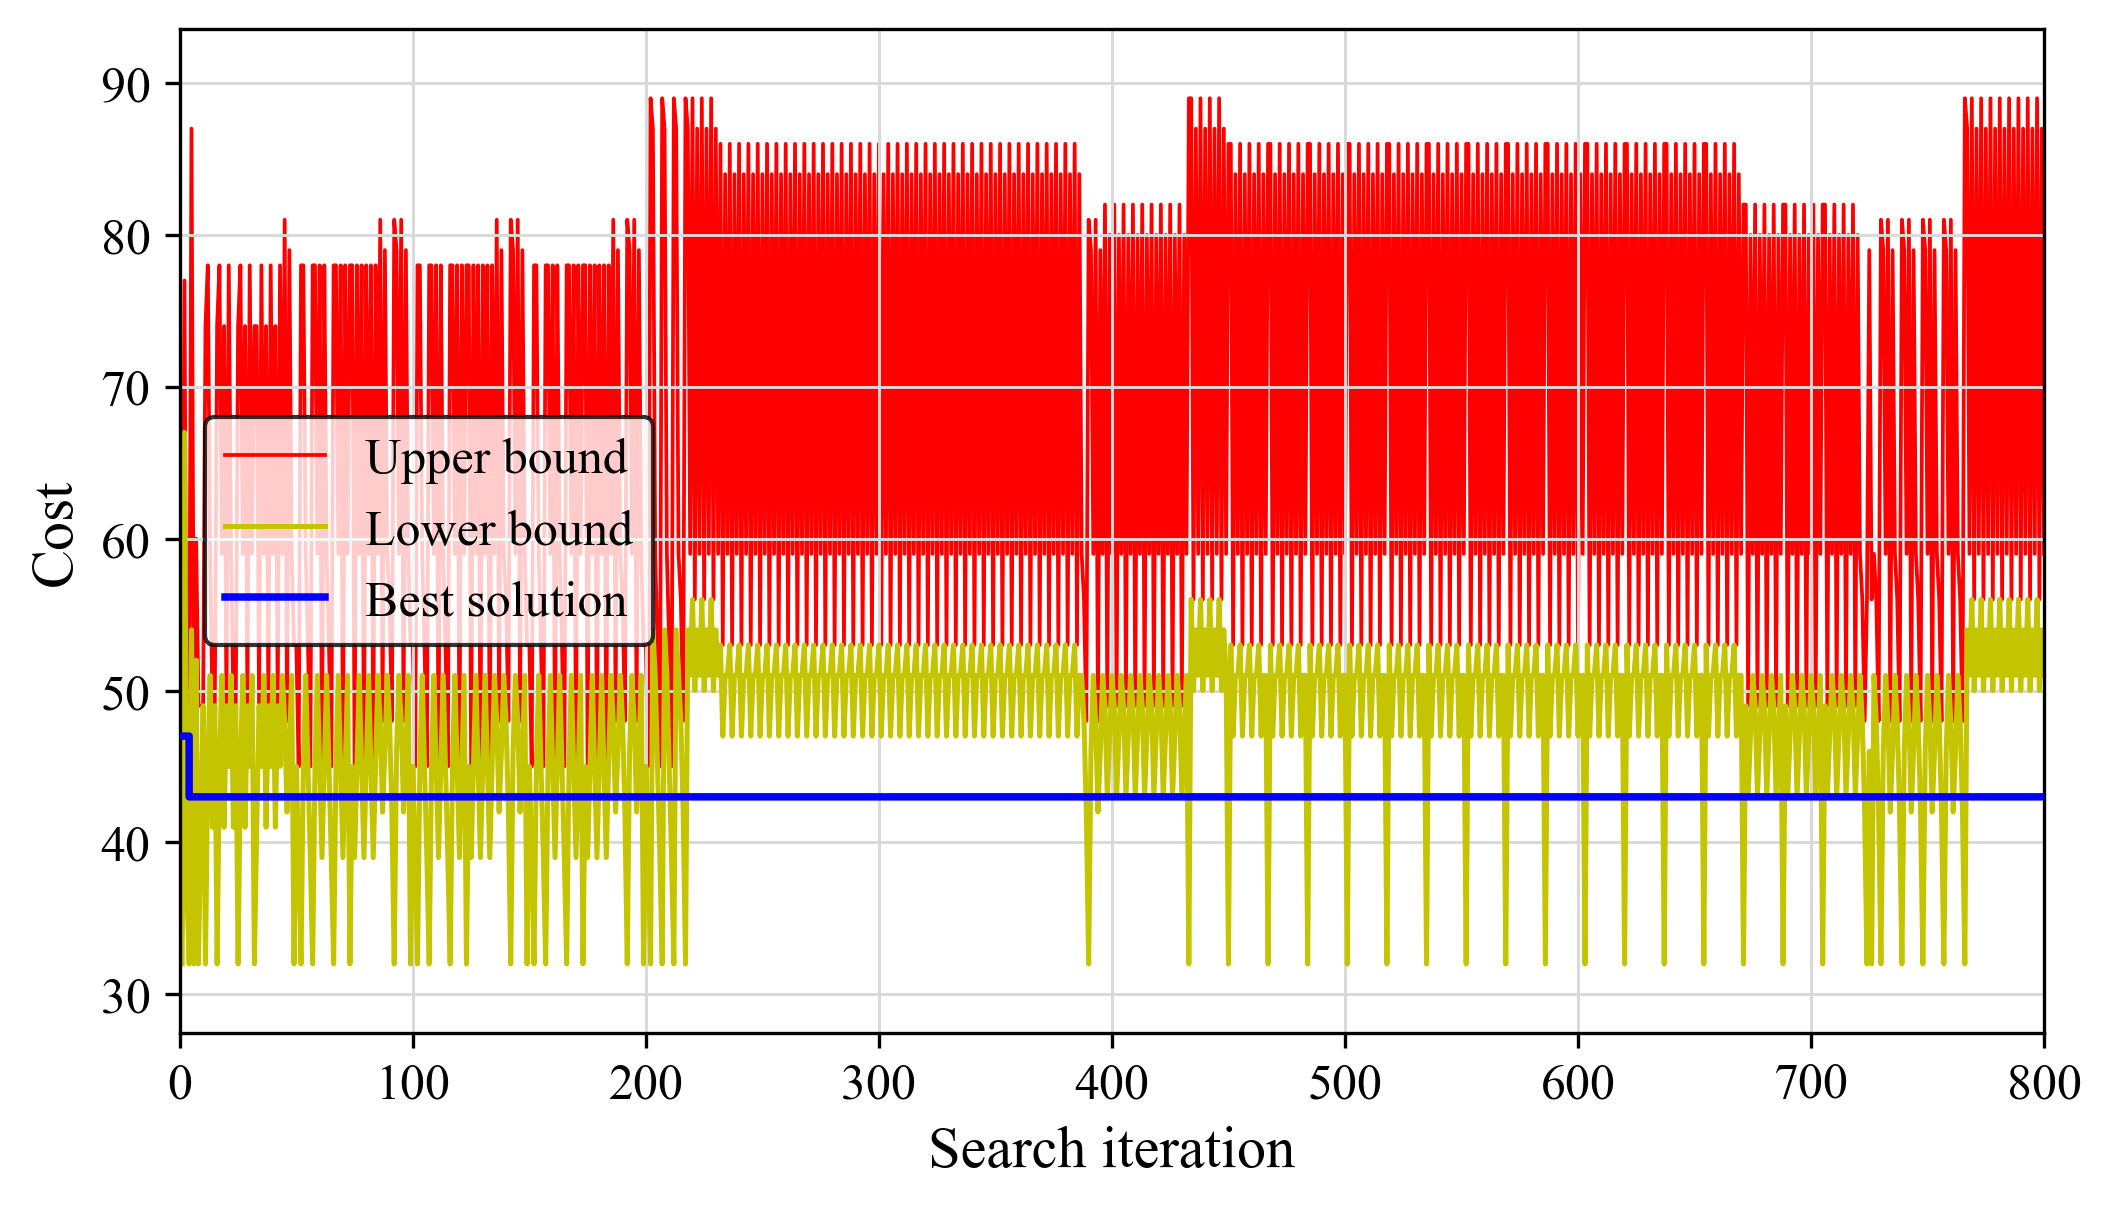
\includegraphics[width=2.5in]{pic/bnb_combo_bounds_first800.png}
\caption{The evolution of the upper bound, lower bound, and optimal value.}
\label{bnb}
\end{figure}


\subsection{Effect of Planning-Aware Automaton Construction}
This case study isolates the contribution of planning-aware automaton construction. We use the same robot team as Sec.\ref{bnb_exp} and consider formulas of the form $\bigwedge_{i=1}^{m}\Diamond a_i$, where $m$ is the number of atomic propositions. Specifically, for $(i=1,\ldots,8)$, $c(a_i)=(1,3,l_i),$ and for $(i=9,\ldots,15)$, $c(a_i)=(2,3,l_{i-8}).$ ]
Thus, $(a_1,\ldots,a_8)$ require three type-1 robots to visit regions $(l_1,\ldots,l_8)$, respectively, while $(a_9,\ldots,a_{15})$ require three type-2 robots to visit regions $(l_1,\ldots,l_7)$, respectively.
The proposed method is compared with two variants. The initial positions of  robots are randomly generated in the workspace. The first variant retains the proposed GBA-level pruning but disables on-the-fly planning, so that planning is performed only after the NBA has been fully constructed. The second variant disables both GBA-level pruning and on-the-fly planning during automaton generation; it first constructs the complete NBA and then applies the same feasibility and decomposability pruning as a post-processing step.

% Table~\ref{tab:early_planning} shows that planning-aware expansion during NBA generation consistently reduces the time to the first feasible solution. For example, when $m=15$, the first-solution time is reduced from 1037.2168 s to 723.6905 s.
% Table~\ref{tab:gba_pruning} further shows that GBA-level
% pruning produces the same pruned NBA size as post-NBA
% pruning, but avoids constructing many redundant transitions in
% the first place. With 15 atomic propositions, the number of
% constructed NBA transitions is reduced from 737,280 to
% 311,296, and the first-solution time decreases from 1235.5359 s
% to 723.6905 s.
% Therefore, the benefit of the proposed framework does not come
% from merely simplifying an already constructed automaton.
% Instead, feasibility and decomposition checks are moved earlier
% in the LTL-to-automaton pipeline, so that unpromising branches
% are prevented from propagating to the NBA and plan-graph
% stages

Tables~\ref{tab:onthefly_planning} and~\ref{tab:early_pruning}  demonstrate the benefit of integrating pruning and planning into the automaton-generation process. Table~\ref{tab:early_planning} isolates the effect of on-the-fly planning when GBA-level pruning is retained. The proposed method consistently obtains the first feasible solution faster than Variant I, which postpones planning until the NBA is fully constructed. This advantage becomes important for longer specifications, because the cost of complete NBA construction grows rapidly with the number of atomic propositions. Instead of waiting for the full NBA, the proposed method constructs the plan graph during NBA generation and can return a feasible plan as soon as an accepting prefix-suffix structure is discovered.

Table~\ref{tab:early_pruning} further shows that early pruning at the GBA level avoids constructing many NBA transitions that would later be removed. For example, when (m=15), Variant II first generates an NBA with ((32768,737280)) states and transitions, whereas the proposed method directly generates the pruned NBA with ((32768,311296)). Although post-processing eventually reduces Variant II to the same NBA size, it has already paid the cost of constructing the larger unpruned NBA. Consequently, its first-solution time is much longer, increasing from 723.6905 s for the proposed method to 1235.5359 s. These results indicate that pruning after complete NBA construction can reduce the final automaton size, but it cannot recover the time wasted on generating unnecessary transitions. Therefore, the proposed framework benefits from both components: GBA-level pruning reduces the automaton construction burden, while on-the-fly planning enables the first feasible plan to be obtained before the complete NBA needs to be explored.

\begin{table}[!t]
\caption{Effect of On-the-Fly Planning on First-Solution Time\label{tab:onthefly_planning}}
\centering
\begin{tabular}{|c||c|c|}
\hline
$m$ & Proposed & Variant I\\
\hline
12 & 10.4065 & 12.7062\\
\hline
13 & 30.7849 & 53.2725\\
\hline
14 & 156.0395 & 197.4069\\
\hline
15 & 723.6905 & 1037.2168\\
\hline
\end{tabular}
\end{table}

\begin{table*}[!t]
\caption{Effect of Early Pruning on NBA Size and First-Solution Time\label{tab:early_pruning}}
\centering
\small
\begin{tabular}{|c||c|c|c|c|c|}
\hline
$m$ & Proposed NBA & Proposed $T_{\mathrm{first}}$ & V-II NBA Before & V-II NBA After & V-II $T_{\mathrm{first}}$\\
\hline
10 & $(1024,6144)$ & 1.0016 & $(1024,10240)$ & $(1024,6144)$ & 1.2243\\
\hline
12 & $(4096,28672)$ & 10.4065 & $(4096,61440)$ & $(4096,28672)$ & 13.5997\\
\hline
13 & $(8192,61440)$ & 30.7849 & $(8192,143360)$ & $(8192,61440)$ & 68.6376\\
\hline
14 & $(16384,131072)$ & 156.0395 & $(16384,327680)$ & $(16384,131072)$ & 239.8623\\
\hline
15 & $(32768,311296)$ & 723.6905 & $(32768,737280)$ & $(32768,311296)$ & 1235.5359\\
\hline
\end{tabular}
\end{table*}
\subsection{First-Solution Quality}
This case study evaluates whether the first feasible solution generated by the on-the-fly plan graph is already of useful quality. Four representative LTL formulas are tested, and each case is executed 25 times. Specifically, we consider
\begin{equation}
\small
\begin{aligned}
\varphi_1 ={}&
\Diamond(a_2 \wedge \Diamond a_1)
\wedge \Diamond(a_3 \wedge \Diamond (a_5 \wedge  \neg p_5) \\
&\wedge \Diamond a_4
\wedge \Diamond a_6
\wedge \Diamond a_7
\wedge \Diamond a_8 ,\\[1mm]
%
\varphi_2 ={}&
\Diamond a_2
\wedge \Diamond a_1
\wedge \Diamond a_3
\wedge \Diamond(a_3 \vee a_4)\\
&\wedge \Diamond a_7
\wedge \Box\Diamond a_5,\\[1mm]
%
\varphi_3 ={}&
\Diamond a_9
\wedge \Diamond a_{10}
\wedge \Diamond(a_3 \wedge a_4)
\wedge \Diamond a_5\\
&\wedge \Box\neg p_1
\wedge \Diamond(a_7 \wedge \Diamond a_8)\\
&\wedge (\neg a_5 \,\mathcal{U}\, (a_3 \wedge a_4)),\\[1mm]
%
\varphi_4 ={}&
\Diamond a_9
\wedge \Diamond a_{10}
\wedge \Diamond a_{11}
\wedge (\neg a_1 \,\mathcal{U}\, a_2)\\
&\wedge \Diamond a_2
\wedge \Diamond a_1
\wedge \Diamond a_5
\wedge \Diamond a_4\\
&\wedge (\Box a_4 \,\mathcal{U}\, a_5).
\end{aligned}
\label{eq:quality_formulas}
\end{equation}
These specifications involve various temporal operators and are representative of complex tasks commonly encountered in large-scale factory scenarios. For example, $\varphi_4$ is adapted from the multi-robot pickup and delivery (MRPD) task\cite{luo2024decomposition}.  Each action proposition $a_i$ is associated with an execution requirement \(c(a_i)=(\tau_i,n_i,l_i)\), where \(\tau_i\) is the required robot type, \(n_i\) is the required number of robots, and \(l_i\) is the target region. Specifically, $ c(a_1) =(2,3,l_1), c(a_2)=(1,2,l_8), c(a_3)=(1,1,l_2),c(a_4)=(2,3,l_4), c(a_5)=(1,3,l_7), c(a_6)=(1,2,l_6),c(a_7)=(1,3,l_7), c(a_8)=(1,3,l_8), c(a_9)=(1,3,l_5),c(a_{10})=(1,3,l_3), c(a_{11})=(1,3,l_1).  $

As shown in Tab.\ref{tab:first_solution_quality}, in two out of four cases, the first solution coincides with the best solution found in the generated plan graph. In the remaining two cases, the first solution is only 1.83\% and 4.47\% worse than the corresponding plan-graph best solution, respectively. Meanwhile, GBA pruning removes 40.24\%-81.48\% of the transitions, and the final graph simplification removes 5.00\%-54.93\% of the plan-graph edges. These results support the residual obligation ordering and shared plan-graph design: the method tends to discover a high-quality executable branch
early while keeping the generated graph compact for subsequent optimization.

\begin{table*}[!t]
\caption{Quality of the First Feasible Solution\label{tab:first_solution_quality}}
\centering
\scriptsize
\begin{tabular}{|c||c|c|c|c|c|c|c|c|}
\hline
\multirow{2}{*}{Case}
& \multicolumn{2}{c|}{First Solution}
& \multicolumn{2}{c|}{Plan-Graph Best}
& \multicolumn{2}{c|}{Global Optimum}
& \multirow{2}{*}{GBA Before/After}
& \multirow{2}{*}{Plan Graph Before/After}\\
\cline{2-7}
& Cost & Time (s)
& Cost & Time (s)
& Cost & Time (s)
& & \\
\hline
1 & 125.23 & 0.1702 & 125.23 & 0.1702 & 102.67 & 1.3557
& $(144,2916)/(144,640)$ & $(712,2232)/(622,1847)$\\
\hline
2 & 74.06 & 0.0619 & 74.06 & 0.0619 & 67.73 & 0.1522
& $(16,82)/(16,49)$ & $(37,60)/(35,57)$\\
\hline
3 & 173.36 & 0.0807 & 170.24 & 0.1071 & 170.24 & 0.1071
& $(36,324)/(20,60)$ & $(43,71)/(22,32)$\\
\hline
4 & 212.98 & 0.4864 & 203.87 & 0.5127 & 176.93 & 1.0008
& $(97,1044)/(81,291)$ & $(212,466)/(131,299)$\\
\hline
\end{tabular}
\end{table*}

% Case Study IV evaluates whether the fast first solution is already of useful quality. Table X reports the first
% solution, the best solution found in the generated plan graph, and the global optimum obtained by
% exhaustive search for small instances. In two out of four cases, the first solution coincides with the best plan-graph solution. In the remaining cases, the first solution is within 1.80\% and 4.28\% of the best plan
% -graph solution, respectively. Meanwhile, GBA pruning removes 40.24\%-81.48\% of transitions and the final
% graph simplification removes 5.00\%-54.93\% of plan-graph edges. These results support the design of the
% residual-obligation ordering and shared plan graph: the method tends to discover a high-quality executable
% branch early while keeping the graph compact enough for subsequent optimization.


\subsection{Scalability}
This case study evaluates scalability with respect to the number of robots. The task formula is $\varphi = \Diamond(a_1 \vee a_2) \wedge\Diamond(a_3 \wedge a_4) \wedge \Diamond a_5 \wedge (\neg a_5\,\mathcal{U}\,(a_3 \wedge a_4))$.  All action propositions in this case require type-1 robots. The execution requirement of each action is defined as \(c(a_i)=(\tau_i,n_i,l_i)\), where \(\tau_i\) is the required robot type, \(n_i\) is the required number of robots, and \(l_i\) is the target region. Specifically, $c(a_1)=(1,n,l_2), c(a_2)=(1,n,l_5),c(a_3)=(1,\lfloor n/3 \rfloor,l_4), c(a_4)=(1,1,l_4), c(a_5)=(1,1,l_5). $
Here, the robot team consists only of type-1 robots, and \(n\) denotes the total number of available type-1 robots. 

Table~\ref{tab:robot_scalability} reports the cost and runtime of the first feasible solution, the best solution found by BnB, and the total search time. The proposed method obtains the first feasible solution quickly for all tested robot-team sizes. Even when (n=100), the first feasible solution is generated in 1.7447 s. This shows that the on-the-fly plan-graph construction remains effective for quickly producing executable plans as the robot team grows.

On the other hand, the total search time increases rapidly with the number of robots. For $n=5$, the search is completed in 12.78 s, while for  $n=20$, it increases to 1426.57 s. When  $n=50$  and  $n=100$, the search is not fully exhausted within the allowed time. This trend is consistent with the complexity analysis. During plan-graph construction, the greedy evaluation of a candidate node grows mainly with the number of compatible robots, so the first-solution time increases moderately. In contrast, the BnB stage must explore robot assignments whose branching factor is bounded by products of combinatorial terms such as $\prod_i \binom{r_i}{k_i}$. As $n$ increases, the number of compatible robots and the required cardinalitie also increase, causing the assignment space to grow combinatorially.

These results demonstrate the anytime nature of the proposed framework. The method can return a feasible solution early even for large robot teams, while additional computation can be used to improve or certify the solution when the assignment space is not too large. For larger teams, complete enumeration becomes difficult, but the planner still provides an executable solution within a short time.

\begin{table}[!t]
\caption{Effect of the Number of Robots\label{tab:robot_scalability}}
\centering
\small
\begin{tabular}{|c||c|c|c|c|c|}
\hline
$n$ & $J_{\mathrm{first}}$ & $T_{\mathrm{first}}$ (s) & $J_{\mathrm{best}}$ & $T_{\mathrm{best}}$ (s) & $T_{\mathrm{search}}$ (s)\\
\hline
5 & 47 & 0.1427 & 43 & 0.6612 & 12.779979\\
\hline
10 & 46 & 0.1977 & 41 & 1.1977 & 263.79\\
\hline
20 & 28 & 0.4176 & 27 & 1.9690 & 1426.57\\
\hline
50 & 22 & 0.8604 & 22 & 0.8604 & $\infty$\\
\hline
100 & 23 & 1.74468 & 23 & 1.74468 & $\infty$\\
\hline
\end{tabular}
\end{table}


\subsection{Comparison With Baselines}
This case study compares the proposed method with a poset-based\cite{liu2024time}method and an MILP-based method\cite{luo2022temporal} on the same LTL formulas and robot-team configurations. The comparison
focuses on both the first-solution latency and the final cost. We consider four LTL specifications:
$$
\begin{aligned}
\varphi_1 ={}&
\Diamond a_1
\wedge \Diamond(a_2 \wedge \Diamond(a_3 \wedge \Diamond a_4))
\wedge \Box\Diamond a_7,\\
\varphi_2 ={}&
\Diamond a_1
\wedge \Diamond a_2
\wedge \Diamond(a_3 \wedge \Diamond(a_6 \wedge \Diamond(a_4 \vee a_5)))\\
&\wedge \Diamond a_7
\wedge \Diamond a_8
\wedge \Diamond(a_9 \wedge \Diamond a_{10}),\\
\varphi_3 ={}&
\Diamond a_1
\wedge \Diamond a_2
\wedge \Diamond(a_3 \wedge \Diamond a_4)
\wedge \Diamond(a_5 \wedge \neg p_7)\\
&\wedge \Diamond a_6
\wedge \Diamond a_9
\wedge (\Box\neg a_9 \mathcal{U} a_6),\\
\varphi_4 ={}&
\Diamond(a_1 \wedge \Diamond a_2)
\wedge \Diamond a_3
\wedge \Diamond a_6
\wedge \Diamond(a_4 \vee a_5)\\
&\wedge \Diamond a_8
\wedge \Diamond a_7
\wedge \Diamond a_9
\wedge \Diamond a_{10}
\wedge (\neg a_9 \mathcal{U} a_2).
\end{aligned}
$$

Specifically, $ c(a_1)=(1,2,l_1), c(a_2)=(2,n,l_2), c(a_3)=(2,1,l_3),c(a_4)=(1,\lfloor n/2 \rfloor,l_4), c(a_5)=(5,\lceil 2n/3 \rceil,l_5), c(a_6)=(3,\max{2,\lceil 0.75n\rceil},l_6),c(a_7)=(1,n,l_7),c(a_8)=(1,2,l_8), c(a_9)=(3,1,l_8),c(a_{10})=(4,1,l_8).$ These specifications are used to evaluate the runtime and solution quality of different methods under increasing task complexity.
The robot team consists of five robot types. We vary  the number of robots of each type $n$ to test different team sizes. For example, let $n = 10$, $5\times 10$ denotes a team with five types of robots and ten robots of each type, i.e., 50 robots in total.

As shown in Tab.\ref{tab:baseline_comparison}, the results show that the proposed method consistently obtains the first feasible solution much faster than the two baselines. This advantage becomes more significant for more complex specifications. For example, under $\varphi_2$ with a $5\times20$ robot team, the proposed method returns the first feasible solution in 1.1497 s, while the poset-based and MILP-based methods require 90.137 s and 67.0037 s, respectively. All three methods eventually reach the same best cost 48.931, but the proposed method reaches its best solution in 3.9071 s, much earlier than the poset-based method and the MILP-based method. Similarly, for the more complex specification $\varphi_4$, the proposed method obtains the first solution within 1.7783 s for the $5\times20$ team, whereas the poset-based and MILP-based methods require 270.42 s and 483.96985 s, respectively.

These results indicate that the proposed framework is particularly effective when an executable plan is needed early. The poset-based method needs to extract and reason over partial-order structures before task allocation, and the MILP-based method must solve a large combinatorial optimization problem before returning a feasible assignment. In contrast, the proposed method constructs the NBA and the plan graph on the fly, so a feasible prefix-suffix plan can be returned as soon as a valid accepting structure is discovered. This explains the large reduction in $T_{\mathrm{first}}$

\begin{table*}[!t]
\caption{Comparison With Poset- and MILP-Based Baselines\label{tab:baseline_comparison}}
\centering
\scriptsize
\setlength{\tabcolsep}{4pt}
\renewcommand{\arraystretch}{1.08}
\begin{tabular}{|c|c|c||c|c|c|c|c|}
\hline
Formula & Team Size & Method 
& $T_{\mathrm{first}}$ (s) 
& $T_{\mathrm{best}}$ (s) 
& $T_{\mathrm{search}}$ (s)
& $J_{\mathrm{first}}$ 
& $J_{\mathrm{best}}$\\
\hline

\multirow{3}{*}{$\varphi_1$} 
& \multirow{3}{*}{$5\times5$}
& Proposed & 0.2104 & 0.3041 & 0.9299 & 57.21 & 51.48\\
\cline{3-8}
& & Poset & 3.3264 & 7.0590 & 11.059 & 58.96 & 51.48\\
\cline{3-8}
& & MILP & 2.1735 & 4.2144 & 59.1163 & 54.38 & 32.85\\
\hline

\multirow{3}{*}{$\varphi_2$} 
& \multirow{3}{*}{$5\times5$}
& Proposed & 0.6987 & 3.9554 & 927.48 & 57.773 & 50.98\\
\cline{3-8}
& & Poset & 89.203 & 91.287 & 940.062 & 62.45 & 50.98\\
\cline{3-8}
& & MILP & 51.4076 & 60.8376 & 632.27 & 66.326 & 50.98\\
\hline

\multirow{3}{*}{$\varphi_2$} 
& \multirow{3}{*}{$5\times10$}
& Proposed & 0.7216 & 4.9678 & 1378.92 & 50.168 & 47.89\\
\cline{3-8}
& & Poset & 89.43 & 92.984 & 1305.835 & 48.78 & 47.89\\
\cline{3-8}
& & MILP & 59.7567 & 62.2364 & 1198.765 & 56.34 & 47.89\\
\hline

\multirow{3}{*}{$\varphi_2$} 
& \multirow{3}{*}{$5\times20$}
& Proposed & 1.1497 & 3.9071 & 8590.59 & 49.987 & 48.931\\
\cline{3-8}
& & Poset & 90.137 & 97.8213 & 8697.43 & 49.076 & 48.931\\
\cline{3-8}
& & MILP & 67.0037 & 74.0153 & 2507.36 & 65.32 & 48.931\\
\hline

\multirow{3}{*}{$\varphi_3$} 
& \multirow{3}{*}{$5\times5$}
& Proposed & 0.3890 & 4.2470 & 157.28 & 38.247 & 33.446\\
\cline{3-8}
& & Poset & 17.921 & 24.587 & 174.114 & 53.32 & 33.446\\
\cline{3-8}
& & MILP & 6.5013 & 11.8756 & 336.4283 & 46.82 & 33.446\\
\hline

\multirow{3}{*}{$\varphi_3$} 
& \multirow{3}{*}{$5\times10$}
& Proposed & 0.3089 & 8.7278 & 203.29 & 35.987 & 32.58\\
\cline{3-8}
& & Poset & 18.385 & 18.985 & 247.815 & 33.48 & 32.58\\
\cline{3-8}
& & MILP & 6.8304 & 13.9769 & 742.93 & 45.32 & 32.58\\
\hline

\multirow{3}{*}{$\varphi_3$} 
& \multirow{3}{*}{$5\times20$}
& Proposed & 0.4203 & 11.8629 & 421.68 & 44.026 & 33.578\\
\cline{3-8}
& & Poset & 17.124 & 24.8491 & 463.769 & 45.7 & 33.578\\
\cline{3-8}
& & MILP & 13.9042 & 18.7462 & 1859.54 & 72.89 & 33.578\\
\hline

\multirow{3}{*}{$\varphi_4$} 
& \multirow{3}{*}{$5\times5$}
& Proposed & 1.3311 & 4.5280 & 9972.67 & 69.46 & 57.42\\
\cline{3-8}
& & Poset & 267.98 & 268.25 & 9903.93 & 67.64 & 57.42\\
\cline{3-8}
& & MILP & 349.1159 & 356.4569 & 1093.42 & 71.326 & 57.42\\
\hline

\multirow{3}{*}{$\varphi_4$} 
& \multirow{3}{*}{$5\times10$}
& Proposed & 1.7716 & 6.8869 & $\infty$ & 47.93 & 35.71\\
\cline{3-8}
& & Poset & 268.98 & 269.54 & $\infty$ & 48.96 & 35.71\\
\cline{3-8}
& & MILP & 371.2282 & 425.7460 & 3467.98 & 84.56 & 35.71\\
\hline

\multirow{3}{*}{$\varphi_4$} 
& \multirow{3}{*}{$5\times20$}
& Proposed & 1.7783 & 7.0542 & $\infty$ & 42.89 & 33.89\\
\cline{3-8}
& & Poset & 270.42 & 271.85 & $\infty$ & 39.67 & 33.89\\
\cline{3-8}
& & MILP & 483.9699 & 508.9515 & 9075.42 & 44.54 & 33.89\\
\hline

\end{tabular}
\end{table*}

\subsection{Online Repair Under Robot Unavailability}
This case study evaluates online repair when the available robot set changes during execution. The original LTL mission remains unchanged, but assignments involving unavailable robots become invalid and the remaining mission must be repaired from the current execution state.  We use the same task specification, AP setting, workspace, and robot-team configuration as in Sec.\ref{bnb_exp}. Two robot-removal events are triggered: robot 0 is removed at $t=15.0$ s and robot 20 is removed at $t=30.0$ s.

The proposed workflow generates repaired first solutions within 45.738 ms and 1.652 ms
for the two events, respectively. The corresponding best repaired solutions are obtained within 69.032 ms and 33.599 ms. As shown in Fig. \ref{dynamic}, during execution, agent 0 breaks down at \(t=15\,\mathrm{s}\) and is removed from the available team. The planner then updates the current execution state and continues the remaining task allocation with the surviving agents. A more severe failure occurs at \(t=30\,\mathrm{s}\), where Agent 20 also becomes unavailable. After this event, the online adaptation module re-identifies the current planning state and resumes the branch-and-bound search from the corresponding node. The unfinished subtasks are then reassigned to the remaining 23 agents. As shown in the timeline figure, no subsequent task segment is assigned to the failed agents, while the remaining agents continue or take over tasks such as \(p_1,p_5\), and \(p_6\). The replanning process preserves the task ordering and collaboration constraints throughout execution. In particular, tasks that are still feasible with the current collaborators continue execution, whereas tasks affected by failed agents are reassigned and executed by other compatible agents. The online search first obtains a feasible solution with cost \(71\), and further improves it to \(62\). Despite the two agent failures, all required tasks are eventually completed at approximately \(62\,\mathrm{s}\), demonstrating that the proposed adaptation method can maintain feasibility and improve the execution plan under unexpected team-size reductions.

\begin{figure}[!t]
\centering
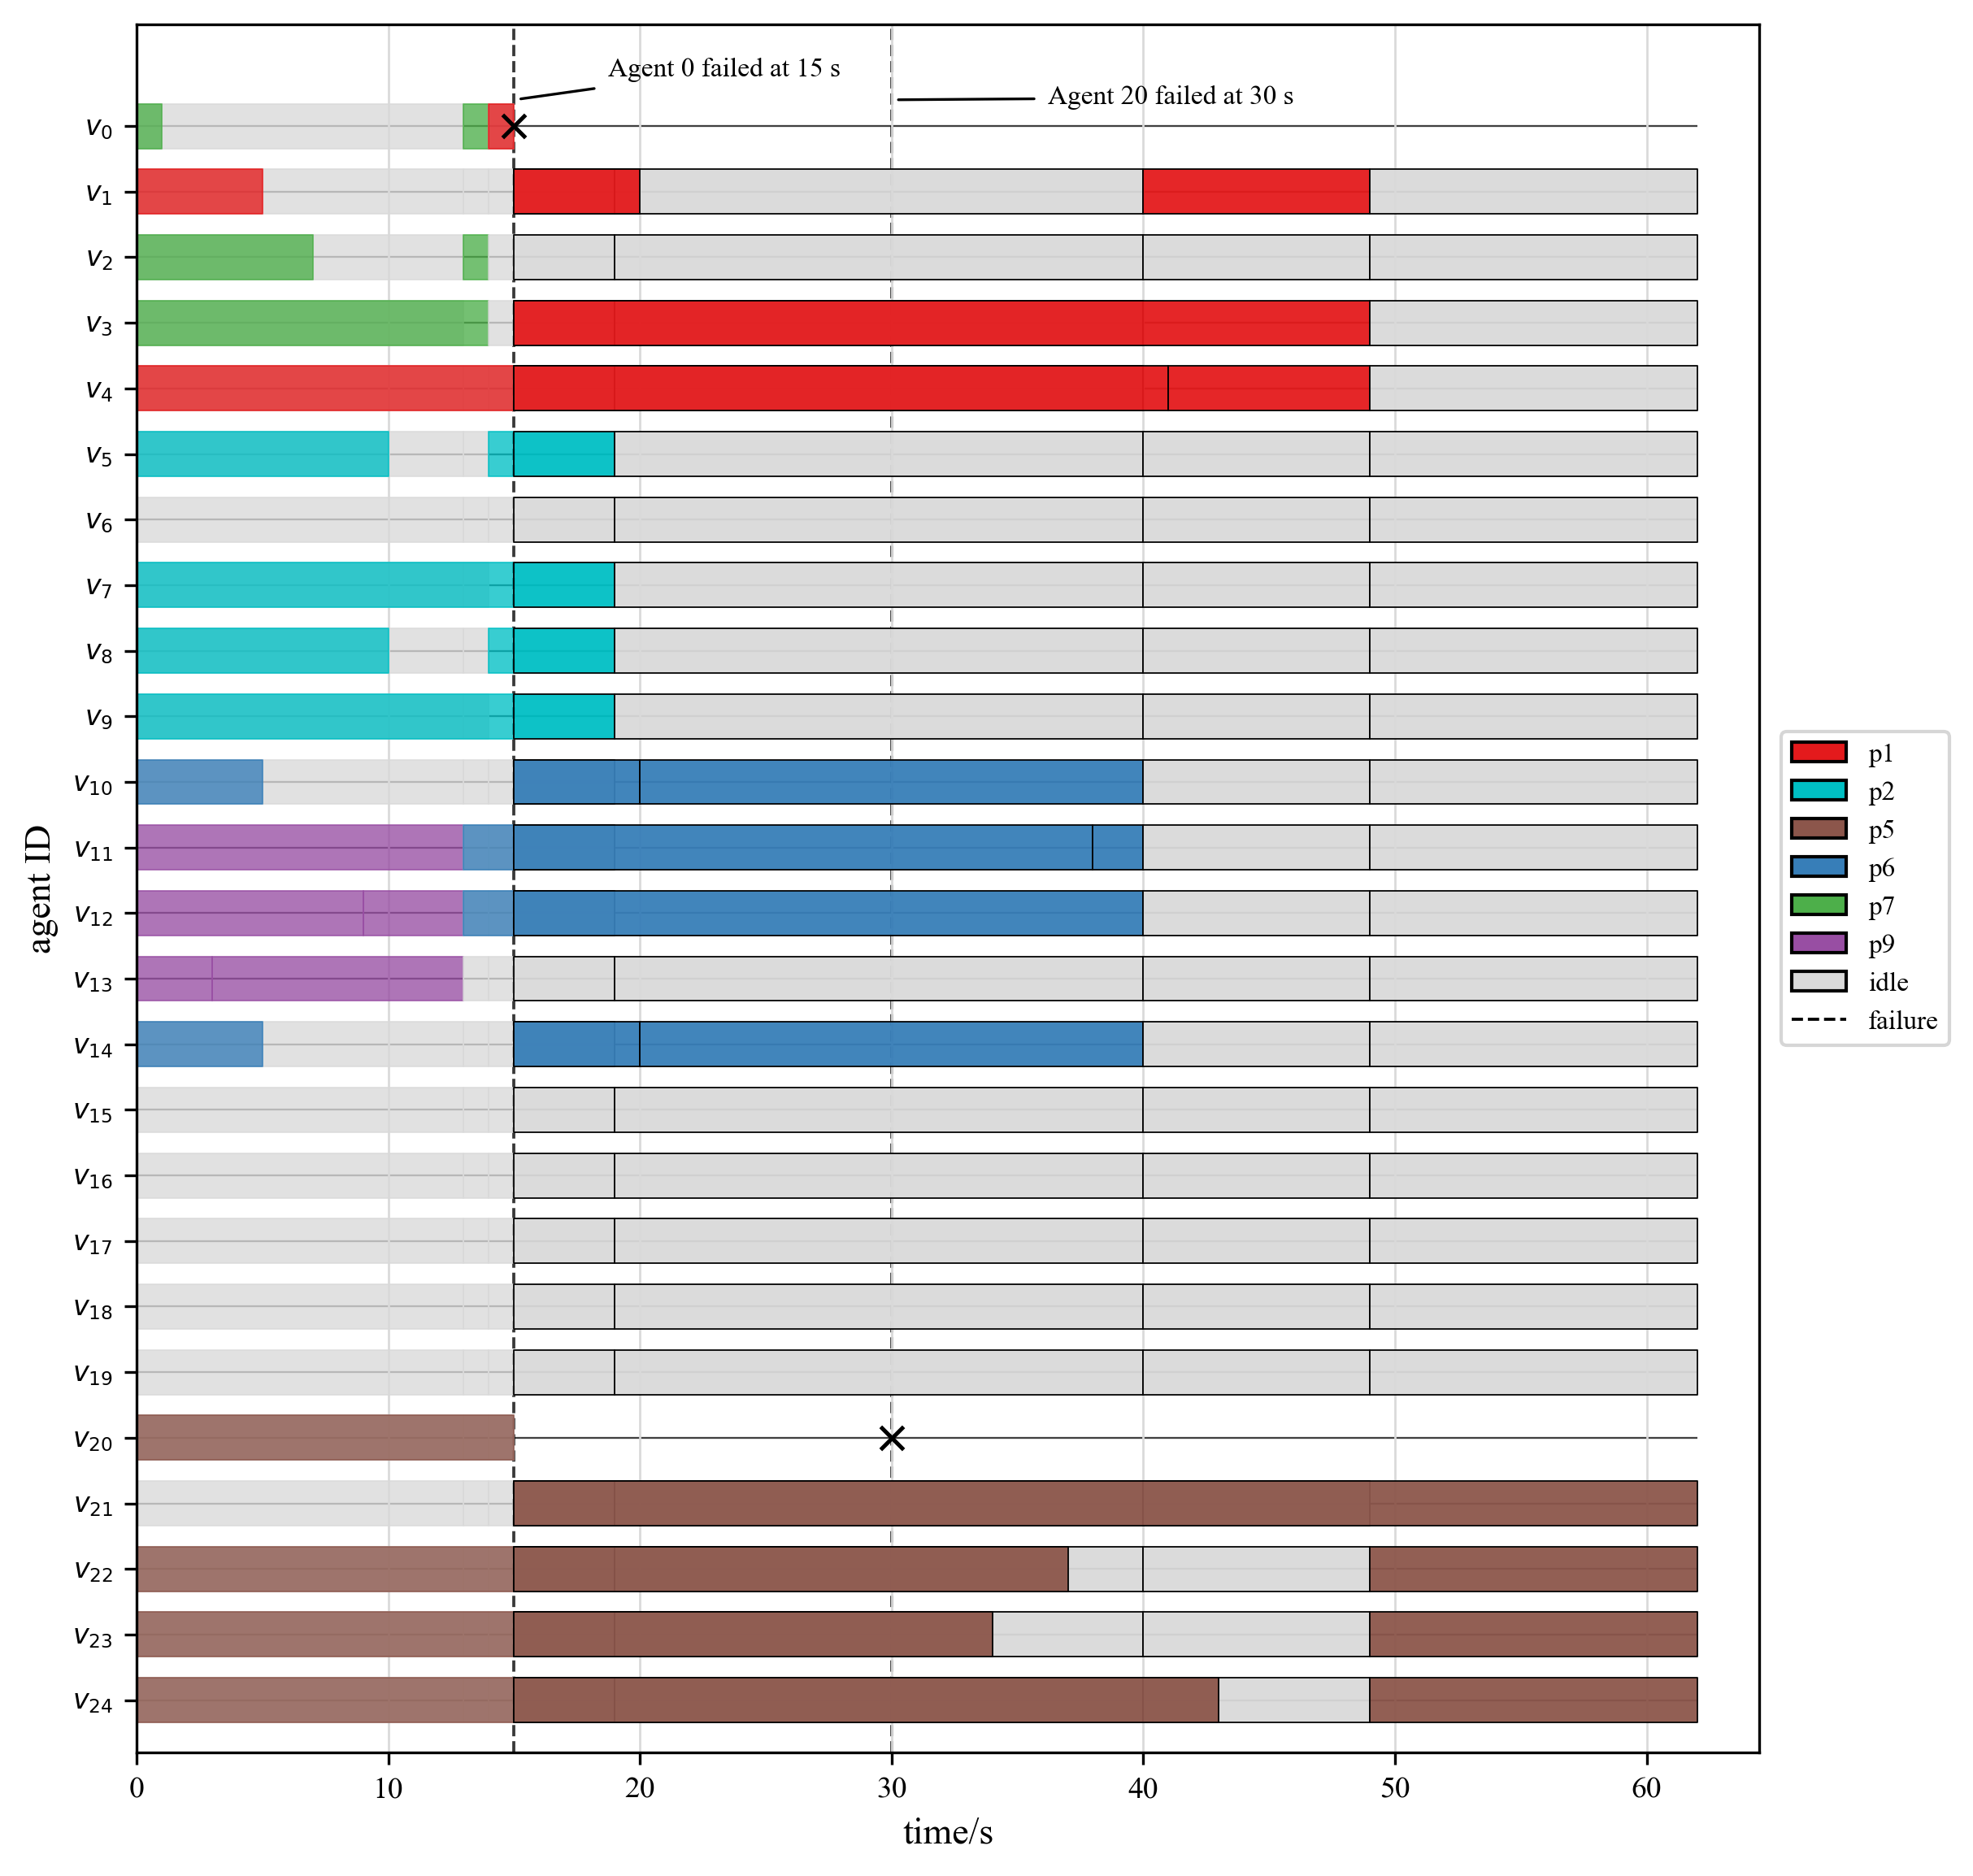
\includegraphics[width=2.5in]{pic/dynamic_robot_timeline_with_idle.png}
\caption{Gantt graph of planning.}
\label{dynamic}
\end{figure}


% \section{The Design, Intent, and \\ Limitations of the Templates}
% The templates are intended to {\bf{approximate the final look and page length of the articles/papers}}. {\bf{They are NOT intended to be the final produced work that is displayed in print or on IEEEXplore\textsuperscript{\textregistered}}}. They will help to give the authors an approximation of the number of pages that will be in the final version. The structure of the \LaTeX\ files, as designed, enable easy conversion to XML for the composition systems used by the IEEE. The XML files are used to produce the final print/IEEEXplore pdf and then converted to HTML for IEEEXplore.

% \section{Where to Get \LaTeX \ Help --- User Groups}
% The following online groups are helpful to beginning and experienced \LaTeX\ users. A search through their archives can provide many answers to common questions.
% \begin{list}{}{}
% \item{\url{http://www.latex-community.org/}} 
% \item{\url{https://tex.stackexchange.com/} }
% \end{list}

% \section{Other Resources}
% See \cite{ref1,ref2,ref3,ref4,ref5} for resources on formatting math into text and additional help in working with \LaTeX .

% \section{Text}
% For some of the remainer of this sample we will use dummy text to fill out paragraphs rather than use live text that may violate a copyright.

% Itam, que ipiti sum dem velit la sum et dionet quatibus apitet voloritet audam, qui aliciant voloreicid quaspe volorem ut maximusandit faccum conemporerum aut ellatur, nobis arcimus.
% Fugit odi ut pliquia incitium latum que cusapere perit molupta eaquaeria quod ut optatem poreiur? Quiaerr ovitior suntiant litio bearciur?

% Onseque sequaes rectur autate minullore nusae nestiberum, sum voluptatio. Et ratem sequiam quaspername nos rem repudandae volum consequis nos eium aut as molupta tectum ulparumquam ut maximillesti consequas quas inctia cum volectinusa porrum unt eius cusaest exeritatur? Nias es enist fugit pa vollum reium essusam nist et pa aceaqui quo elibusdandis deligendus que nullaci lloreri bla que sa coreriam explacc atiumquos simolorpore, non prehendunt lam que occum\cite{ref6} si aut aut maximus eliaeruntia dia sequiamenime natem sendae ipidemp orehend uciisi omnienetus most verum, ommolendi omnimus, est, veni aut ipsa volendelist mo conserum volores estisciis recessi nveles ut poressitatur sitiis ex endi diti volum dolupta aut aut odi as eatquo cullabo remquis toreptum et des accus dolende pores sequas dolores tinust quas expel moditae ne sum quiatis nis endipie nihilis etum fugiae audi dia quiasit quibus.
% \IEEEpubidadjcol
% Ibus el et quatemo luptatque doluptaest et pe volent rem ipidusa eribus utem venimolorae dera qui acea quam etur aceruptat.
% Gias anis doluptaspic tem et aliquis alique inctiuntiur?

% Sedigent, si aligend elibuscid ut et ium volo tem eictore pellore ritatus ut ut ullatus in con con pere nos ab ium di tem aliqui od magnit repta volectur suntio. Nam isquiante doluptis essit, ut eos suntionsecto debitiur sum ea ipitiis adipit, oditiore, a dolorerempos aut harum ius, atquat.

% Rum rem ditinti sciendunti volupiciendi sequiae nonsect oreniatur, volores sition ressimil inus solut ea volum harumqui to see\eqref{deqn_ex1a} mint aut quat eos explis ad quodi debis deliqui aspel earcius.

% \begin{equation}
% \label{deqn_ex1a}
% x = \sum_{i=0}^{n} 2{i} Q.
% \end{equation}

% Alis nime volorempera perferi sitio denim repudae pre ducilit atatet volecte ssimillorae dolore, ut pel ipsa nonsequiam in re nus maiost et que dolor sunt eturita tibusanis eatent a aut et dio blaudit reptibu scipitem liquia consequodi od unto ipsae. Et enitia vel et experferum quiat harum sa net faccae dolut voloria nem. Bus ut labo. Ita eum repraer rovitia samendit aut et volupta tecupti busant omni quiae porro que nossimodic temquis anto blacita conse nis am, que ereperum eumquam quaescil imenisci quae magnimos recus ilibeaque cum etum iliate prae parumquatemo blaceaquiam quundia dit apienditem rerit re eici quaes eos sinvers pelecabo. Namendignis as exerupit aut magnim ium illabor roratecte plic tem res apiscipsam et vernat untur a deliquaest que non cus eat ea dolupiducim fugiam volum hil ius dolo eaquis sitis aut landesto quo corerest et auditaquas ditae voloribus, qui optaspis exero cusa am, ut plibus.


% \section{Some Common Elements}
% \subsection{Sections and Subsections}
% Enumeration of section headings is desirable, but not required. When numbered, please be consistent throughout the article, that is, all headings and all levels of section headings in the article should be enumerated. Primary headings are designated with Roman numerals, secondary with capital letters, tertiary with Arabic numbers; and quaternary with lowercase letters. Reference and Acknowledgment headings are unlike all other section headings in text. They are never enumerated. They are simply primary headings without labels, regardless of whether the other headings in the article are enumerated. 

% \subsection{Citations to the Bibliography}
% The coding for the citations is made with the \LaTeX\ $\backslash${\tt{cite}} command. 
% This will display as: see \cite{ref1}.

% For multiple citations code as follows: {\tt{$\backslash$cite\{ref1,ref2,ref3\}}}
%  which will produce \cite{ref1,ref2,ref3}. For reference ranges that are not consecutive code as {\tt{$\backslash$cite\{ref1,ref2,ref3,ref9\}}} which will produce  \cite{ref1,ref2,ref3,ref9}

% \subsection{Lists}
% In this section, we will consider three types of lists: simple unnumbered, numbered, and bulleted. There have been many options added to IEEEtran to enhance the creation of lists. If your lists are more complex than those shown below, please refer to the original ``IEEEtran\_HOWTO.pdf'' for additional options.\\

% \subsubsection*{\bf A plain  unnumbered list}
% \begin{list}{}{}
% \item{bare\_jrnl.tex}
% \item{bare\_conf.tex}
% \item{bare\_jrnl\_compsoc.tex}
% \item{bare\_conf\_compsoc.tex}
% \item{bare\_jrnl\_comsoc.tex}
% \end{list}

% \subsubsection*{\bf A simple numbered list}
% \begin{enumerate}
% \item{bare\_jrnl.tex}
% \item{bare\_conf.tex}
% \item{bare\_jrnl\_compsoc.tex}
% \item{bare\_conf\_compsoc.tex}
% \item{bare\_jrnl\_comsoc.tex}
% \end{enumerate}

% \subsubsection*{\bf A simple bulleted list}
% \begin{itemize}
% \item{bare\_jrnl.tex}
% \item{bare\_conf.tex}
% \item{bare\_jrnl\_compsoc.tex}
% \item{bare\_conf\_compsoc.tex}
% \item{bare\_jrnl\_comsoc.tex}
% \end{itemize}





% \subsection{Figures}
% Fig. 1 is an example of a floating figure using the graphicx package.
%  Note that $\backslash${\tt{label}} must occur AFTER (or within) $\backslash${\tt{caption}}.
%  For figures, $\backslash${\tt{caption}} should occur after the $\backslash${\tt{includegraphics}}.

% \begin{figure}[!t]
% \centering
% 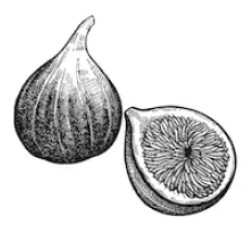
\includegraphics[width=2.5in]{fig1}
% \caption{Simulation results for the network.}
% \label{fig_1}
% \end{figure}

% Fig. 2(a) and 2(b) is an example of a double column floating figure using two subfigures.
%  (The subfig.sty package must be loaded for this to work.)
%  The subfigure $\backslash${\tt{label}} commands are set within each subfloat command,
%  and the $\backslash${\tt{label}} for the overall figure must come after $\backslash${\tt{caption}}.
%  $\backslash${\tt{hfil}} is used as a separator to get equal spacing.
%  The combined width of all the parts of the figure should do not exceed the text width or a line break will occur.
% %
% \begin{figure*}[!t]
% \centering
% \subfloat[]{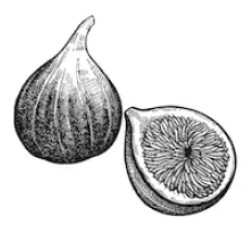
\includegraphics[width=2.5in]{fig1}%
% \label{fig_first_case}}
% \hfil
% \subfloat[]{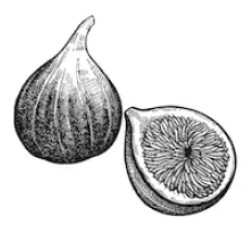
\includegraphics[width=2.5in]{fig1}%
% \label{fig_second_case}}
% \caption{Dae. Ad quatur autat ut porepel itemoles dolor autem fuga. Bus quia con nessunti as remo di quatus non perum que nimus. (a) Case I. (b) Case II.}
% \label{fig_sim}
% \end{figure*}

% Note that often IEEE papers with multi-part figures do not place the labels within the image itself (using the optional argument to $\backslash${\tt{subfloat}}[]), but instead will
%  reference/describe all of them (a), (b), etc., within the main caption.
%  Be aware that for subfig.sty to generate the (a), (b), etc., subfigure
%  labels, the optional argument to $\backslash${\tt{subfloat}} must be present. If a
%  subcaption is not desired, leave its contents blank,
%  e.g.,$\backslash${\tt{subfloat}}[].


 

% \section{Tables}
% Note that, for IEEE-style tables, the
%  $\backslash${\tt{caption}} command should come BEFORE the table. Table captions use title case. Articles (a, an, the), coordinating conjunctions (and, but, for, or, nor), and most short prepositions are lowercase unless they are the first or last word. Table text will default to $\backslash${\tt{footnotesize}} as
%  the IEEE normally uses this smaller font for tables.
%  The $\backslash${\tt{label}} must come after $\backslash${\tt{caption}} as always.
 
% \begin{table}[!t]
% \caption{An Example of a Table\label{tab:table1}}
% \centering
% \begin{tabular}{|c||c|}
% \hline
% One & Two\\
% \hline
% Three & Four\\
% \hline
% \end{tabular}
% \end{table}

% \section{Algorithms}
% Algorithms should be numbered and include a short title. They are set off from the text with rules above and below the title and after the last line.

% \begin{algorithm}[H]
% \caption{Weighted Tanimoto ELM.}\label{alg:alg1}
% \begin{algorithmic}
% \STATE 
% \STATE {\textsc{TRAIN}}$(\mathbf{X} \mathbf{T})$
% \STATE \hspace{0.5cm}$ \textbf{select randomly } W \subset \mathbf{X}  $
% \STATE \hspace{0.5cm}$ N_\mathbf{t} \gets | \{ i : \mathbf{t}_i = \mathbf{t} \} | $ \textbf{ for } $ \mathbf{t}= -1,+1 $
% \STATE \hspace{0.5cm}$ B_i \gets \sqrt{ \textsc{max}(N_{-1},N_{+1}) / N_{\mathbf{t}_i} } $ \textbf{ for } $ i = 1,...,N $
% \STATE \hspace{0.5cm}$ \hat{\mathbf{H}} \gets  B \cdot (\mathbf{X}^T\textbf{W})/( \mathbb{1}\mathbf{X} + \mathbb{1}\textbf{W} - \mathbf{X}^T\textbf{W} ) $
% \STATE \hspace{0.5cm}$ \beta \gets \left ( I/C + \hat{\mathbf{H}}^T\hat{\mathbf{H}} \right )^{-1}(\hat{\mathbf{H}}^T B\cdot \mathbf{T})  $
% \STATE \hspace{0.5cm}\textbf{return}  $\textbf{W},  \beta $
% \STATE 
% \STATE {\textsc{PREDICT}}$(\mathbf{X} )$
% \STATE \hspace{0.5cm}$ \mathbf{H} \gets  (\mathbf{X}^T\textbf{W} )/( \mathbb{1}\mathbf{X}  + \mathbb{1}\textbf{W}- \mathbf{X}^T\textbf{W}  ) $
% \STATE \hspace{0.5cm}\textbf{return}  $\textsc{sign}( \mathbf{H} \beta )$
% \end{algorithmic}
% \label{alg1}
% \end{algorithm}

% Que sunt eum lam eos si dic to estist, culluptium quid qui nestrum nobis reiumquiatur minimus minctem. Ro moluptat fuga. Itatquiam ut laborpo rersped exceres vollandi repudaerem. Ulparci sunt, qui doluptaquis sumquia ndestiu sapient iorepella sunti veribus. Ro moluptat fuga. Itatquiam ut laborpo rersped exceres vollandi repudaerem. 
% \section{Mathematical Typography \\ and Why It Matters}

% Typographical conventions for mathematical formulas have been developed to {\bf provide uniformity and clarity of presentation across mathematical texts}. This enables the readers of those texts to both understand the author's ideas and to grasp new concepts quickly. While software such as \LaTeX \ and MathType\textsuperscript{\textregistered} can produce aesthetically pleasing math when used properly, it is also very easy to misuse the software, potentially resulting in incorrect math display.

% IEEE aims to provide authors with the proper guidance on mathematical typesetting style and assist them in writing the best possible article. As such, IEEE has assembled a set of examples of good and bad mathematical typesetting \cite{ref1,ref2,ref3,ref4,ref5}. 

% Further examples can be found at \url{http://journals.ieeeauthorcenter.ieee.org/wp-content/uploads/sites/7/IEEE-Math-Typesetting-Guide-for-LaTeX-Users.pdf}

% \subsection{Display Equations}
% The simple display equation example shown below uses the ``equation'' environment. To number the equations, use the $\backslash${\tt{label}} macro to create an identifier for the equation. LaTeX will automatically number the equation for you.
% \begin{equation}
% \label{deqn_ex1}
% x = \sum_{i=0}^{n} 2{i} Q.
% \end{equation}

% \noindent is coded as follows:
% \begin{verbatim}
% \begin{equation}
% \label{deqn_ex1}
% x = \sum_{i=0}^{n} 2{i} Q.
% \end{equation}
% \end{verbatim}

% To reference this equation in the text use the $\backslash${\tt{ref}} macro. 
% Please see (\ref{deqn_ex1})\\
% \noindent is coded as follows:
% \begin{verbatim}
% Please see (\ref{deqn_ex1})\end{verbatim}

% \subsection{Equation Numbering}
% {\bf{Consecutive Numbering:}} Equations within an article are numbered consecutively from the beginning of the
% article to the end, i.e., (1), (2), (3), (4), (5), etc. Do not use roman numerals or section numbers for equation numbering.

% \noindent {\bf{Appendix Equations:}} The continuation of consecutively numbered equations is best in the Appendix, but numbering
%  as (A1), (A2), etc., is permissible.\\

% \noindent {\bf{Hyphens and Periods}}: Hyphens and periods should not be used in equation numbers, i.e., use (1a) rather than
% (1-a) and (2a) rather than (2.a) for subequations. This should be consistent throughout the article.

% \subsection{Multi-Line Equations and Alignment}
% Here we show several examples of multi-line equations and proper alignments.

% \noindent {\bf{A single equation that must break over multiple lines due to length with no specific alignment.}}
% \begin{multline}
% \text{The first line of this example}\\
% \text{The second line of this example}\\
% \text{The third line of this example}
% \end{multline}

% \noindent is coded as:
% \begin{verbatim}
% \begin{multline}
% \text{The first line of this example}\\
% \text{The second line of this example}\\
% \text{The third line of this example}
% \end{multline}
% \end{verbatim}

% \noindent {\bf{A single equation with multiple lines aligned at the = signs}}
% \begin{align}
% a &= c+d \\
% b &= e+f
% \end{align}
% \noindent is coded as:
% \begin{verbatim}
% \begin{align}
% a &= c+d \\
% b &= e+f
% \end{align}
% \end{verbatim}

% The {\tt{align}} environment can align on multiple  points as shown in the following example:
% \begin{align}
% x &= y & X & =Y & a &=bc\\
% x' &= y' & X' &=Y' &a' &=bz
% \end{align}
% \noindent is coded as:
% \begin{verbatim}
% \begin{align}
% x &= y & X & =Y & a &=bc\\
% x' &= y' & X' &=Y' &a' &=bz
% \end{align}
% \end{verbatim}





% \subsection{Subnumbering}
% The amsmath package provides a {\tt{subequations}} environment to facilitate subnumbering. An example:

% \begin{subequations}\label{eq:2}
% \begin{align}
% f&=g \label{eq:2A}\\
% f' &=g' \label{eq:2B}\\
% \mathcal{L}f &= \mathcal{L}g \label{eq:2c}
% \end{align}
% \end{subequations}

% \noindent is coded as:
% \begin{verbatim}
% \begin{subequations}\label{eq:2}
% \begin{align}
% f&=g \label{eq:2A}\\
% f' &=g' \label{eq:2B}\\
% \mathcal{L}f &= \mathcal{L}g \label{eq:2c}
% \end{align}
% \end{subequations}

% \end{verbatim}

% \subsection{Matrices}
% There are several useful matrix environments that can save you some keystrokes. See the example coding below and the output.

% \noindent {\bf{A simple matrix:}}
% \begin{equation}
% \begin{matrix}  0 &  1 \\ 
% 1 &  0 \end{matrix}
% \end{equation}
% is coded as:
% \begin{verbatim}
% \begin{equation}
% \begin{matrix}  0 &  1 \\ 
% 1 &  0 \end{matrix}
% \end{equation}
% \end{verbatim}

% \noindent {\bf{A matrix with parenthesis}}
% \begin{equation}
% \begin{pmatrix} 0 & -i \\
%  i &  0 \end{pmatrix}
% \end{equation}
% is coded as:
% \begin{verbatim}
% \begin{equation}
% \begin{pmatrix} 0 & -i \\
%  i &  0 \end{pmatrix}
% \end{equation}
% \end{verbatim}

% \noindent {\bf{A matrix with square brackets}}
% \begin{equation}
% \begin{bmatrix} 0 & -1 \\ 
% 1 &  0 \end{bmatrix}
% \end{equation}
% is coded as:
% \begin{verbatim}
% \begin{equation}
% \begin{bmatrix} 0 & -1 \\ 
% 1 &  0 \end{bmatrix}
% \end{equation}
% \end{verbatim}

% \noindent {\bf{A matrix with curly braces}}
% \begin{equation}
% \begin{Bmatrix} 1 &  0 \\ 
% 0 & -1 \end{Bmatrix}
% \end{equation}
% is coded as:
% \begin{verbatim}
% \begin{equation}
% \begin{Bmatrix} 1 &  0 \\ 
% 0 & -1 \end{Bmatrix}
% \end{equation}\end{verbatim}

% \noindent {\bf{A matrix with single verticals}}
% \begin{equation}
% \begin{vmatrix} a &  b \\ 
% c &  d \end{vmatrix}
% \end{equation}
% is coded as:
% \begin{verbatim}
% \begin{equation}
% \begin{vmatrix} a &  b \\ 
% c &  d \end{vmatrix}
% \end{equation}\end{verbatim}

% \noindent {\bf{A matrix with double verticals}}
% \begin{equation}
% \begin{Vmatrix} i &  0 \\ 
% 0 & -i \end{Vmatrix}
% \end{equation}
% is coded as:
% \begin{verbatim}
% \begin{equation}
% \begin{Vmatrix} i &  0 \\ 
% 0 & -i \end{Vmatrix}
% \end{equation}\end{verbatim}

% \subsection{Arrays}
% The {\tt{array}} environment allows you some options for matrix-like equations. You will have to manually key the fences, but there are other options for alignment of the columns and for setting horizontal and vertical rules. The argument to {\tt{array}} controls alignment and placement of vertical rules.

% A simple array
% \begin{equation}
% \left(
% \begin{array}{cccc}
% a+b+c & uv & x-y & 27\\
% a+b & u+v & z & 134
% \end{array}\right)
% \end{equation}
% is coded as:
% \begin{verbatim}
% \begin{equation}
% \left(
% \begin{array}{cccc}
% a+b+c & uv & x-y & 27\\
% a+b & u+v & z & 134
% \end{array} \right)
% \end{equation}
% \end{verbatim}

% A slight variation on this to better align the numbers in the last column
% \begin{equation}
% \left(
% \begin{array}{cccr}
% a+b+c & uv & x-y & 27\\
% a+b & u+v & z & 134
% \end{array}\right)
% \end{equation}
% is coded as:
% \begin{verbatim}
% \begin{equation}
% \left(
% \begin{array}{cccr}
% a+b+c & uv & x-y & 27\\
% a+b & u+v & z & 134
% \end{array} \right)
% \end{equation}
% \end{verbatim}

% An array with vertical and horizontal rules
% \begin{equation}
% \left( \begin{array}{c|c|c|r}
% a+b+c & uv & x-y & 27\\ \hline
% a+b & u+v & z & 134
% \end{array}\right)
% \end{equation}
% is coded as:
% \begin{verbatim}
% \begin{equation}
% \left(
% \begin{array}{c|c|c|r}
% a+b+c & uv & x-y & 27\\
% a+b & u+v & z & 134
% \end{array} \right)
% \end{equation}
% \end{verbatim}
% Note the argument now has the pipe "$\vert$" included to indicate the placement of the vertical rules.


% \subsection{Cases Structures}
% Many times cases can be miscoded using the wrong environment, i.e., {\tt{array}}. Using the {\tt{cases}} environment will save keystrokes (from not having to type the $\backslash${\tt{left}}$\backslash${\tt{lbrace}}) and automatically provide the correct column alignment.
% \begin{equation*}
% {z_m(t)} = \begin{cases}
% 1,&{\text{if}}\ {\beta }_m(t) \\ 
% {0,}&{\text{otherwise.}} 
% \end{cases}
% \end{equation*}
% \noindent is coded as follows:
% \begin{verbatim}
% \begin{equation*}
% {z_m(t)} = 
% \begin{cases}
% 1,&{\text{if}}\ {\beta }_m(t),\\ 
% {0,}&{\text{otherwise.}} 
% \end{cases}
% \end{equation*}
% \end{verbatim}
% \noindent Note that the ``\&'' is used to mark the tabular alignment. This is important to get  proper column alignment. Do not use $\backslash${\tt{quad}} or other fixed spaces to try and align the columns. Also, note the use of the $\backslash${\tt{text}} macro for text elements such as ``if'' and ``otherwise.''

% \subsection{Function Formatting in Equations}
% Often, there is an easy way to properly format most common functions. Use of the $\backslash$ in front of the function name will in most cases, provide the correct formatting. When this does not work, the following example provides a solution using the $\backslash${\tt{text}} macro:

% \begin{equation*} 
%   d_{R}^{KM} = \underset {d_{l}^{KM}} {\text{arg min}} \{ d_{1}^{KM},\ldots,d_{6}^{KM}\}.
% \end{equation*}

% \noindent is coded as follows:
% \begin{verbatim}
% \begin{equation*} 
%  d_{R}^{KM} = \underset {d_{l}^{KM}} 
%  {\text{arg min}} \{ d_{1}^{KM},
%  \ldots,d_{6}^{KM}\}.
% \end{equation*}
% \end{verbatim}

% \subsection{ Text Acronyms Inside Equations}
% This example shows where the acronym ``MSE" is coded using $\backslash${\tt{text\{\}}} to match how it appears in the text.

% \begin{equation*}
%  \text{MSE} = \frac {1}{n}\sum _{i=1}^{n}(Y_{i} - \hat {Y_{i}})^{2}
% \end{equation*}

% \begin{verbatim}
% \begin{equation*}
%  \text{MSE} = \frac {1}{n}\sum _{i=1}^{n}
% (Y_{i} - \hat {Y_{i}})^{2}
% \end{equation*}
% \end{verbatim}
\section{Physical experiments}

\section{Conclusion}
In this work, a novel on-the-fly planning framework has been proposed for temporal-logic task allocation in heterogeneous multi-robot systems. The framework performs task allocation during score-guided NBA construction and uses GBA-level pruning to obtain an executable solution early. A branch-and-bound procedure further improves the solution. In addition, an online replanning strategy reassigns unfinished tasks when robots become unavailable. Theoretical analysis establishes completeness of our algorithm.
Numerical and physical experiments validate the efficiency, solution quality, scalability, and adaptability of the proposed framework.


\section*{Acknowledgments}
This should be a simple paragraph before the References to thank those individuals and institutions who have supported your work on this article.



% {\appendix[Proof of the Zonklar Equations]
% Use $\backslash${\tt{appendix}} if you have a single appendix:
% Do not use $\backslash${\tt{section}} anymore after $\backslash${\tt{appendix}}, only $\backslash${\tt{section*}}.
% If you have multiple appendixes use $\backslash${\tt{appendices}} then use $\backslash${\tt{section}} to start each appendix.
% You must declare a $\backslash${\tt{section}} before using any $\backslash${\tt{subsection}} or using $\backslash${\tt{label}} ($\backslash${\tt{appendices}} by itself
%  starts a section numbered zero.)}



% %{\appendices
% %\section*{Proof of the First Zonklar Equation}
% %Appendix one text goes here.
% % You can choose not to have a title for an appendix if you want by leaving the argument blank
% %\section*{Proof of the Second Zonklar Equation}
% %Appendix two text goes here.}



% \section{References Section}
% You can use a bibliography generated by BibTeX as a .bbl file.
%  BibTeX documentation can be easily obtained at:
%  http://mirror.ctan.org/biblio/bibtex/contrib/doc/
%  The IEEEtran BibTeX style support page is:
%  http://www.michaelshell.org/tex/ieeetran/bibtex/
 
 % argument is your BibTeX string definitions and bibliography database(s)
%\bibliography{IEEEabrv,../bib/paper}
%
% \section{Simple References}
% You can manually copy in the resultant .bbl file and set second argument of $\backslash${\tt{begin}} to the number of references
%  (used to reserve space for the reference number labels box).
%
% \begin{thebibliography}{1}
% \bibliographystyle{IEEEtran}
%
% \bibitem{ref1}
% {\it{Mathematics Into Type}}. American Mathematical Society. [Online]. Available: https://www.ams.org/arc/styleguide/mit-2.pdf
%
% \bibitem{ref2}
% T. W. Chaundy, P. R. Barrett and C. Batey, {\it{The Printing of Mathematics}}. London, U.K., Oxford Univ. Press, 1954.
%
% \bibitem{ref3}
% F. Mittelbach and M. Goossens, {\it{The \LaTeX Companion}}, 2nd ed. Boston, MA, USA: Pearson, 2004.
%
% \bibitem{ref4}
% G. Gr\"atzer, {\it{More Math Into LaTeX}}, New York, NY, USA: Springer, 2007.
%
% \bibitem{ref5}M. Letourneau and J. W. Sharp, {\it{AMS-StyleGuide-online.pdf,}} American Mathematical Society, Providence, RI, USA, [Online]. Available: http://www.ams.org/arc/styleguide/index.html
%
% \bibitem{ref6}
% H. Sira-Ramirez, ``On the sliding mode control of nonlinear systems,'' \textit{Syst. Control Lett.}, vol. 19, pp. 303--312, 1992.
%
% \bibitem{ref7}
% A. Levant, ``Exact differentiation of signals with unbounded higher derivatives,''  in \textit{Proc. 45th IEEE Conf. Decis.
% Control}, San Diego, CA, USA, 2006, pp. 5585--5590. DOI: 10.1109/CDC.2006.377165.
%
% \bibitem{ref8}
% M. Fliess, C. Join, and H. Sira-Ramirez, ``Non-linear estimation is easy,'' \textit{Int. J. Model., Ident. Control}, vol. 4, no. 1, pp. 12--27, 2008.
%
% \bibitem{ref9}
% R. Ortega, A. Astolfi, G. Bastin, and H. Rodriguez, ``Stabilization of food-chain systems using a port-controlled Hamiltonian description,'' in \textit{Proc. Amer. Control Conf.}, Chicago, IL, USA,
% 2000, pp. 2245--2249.
%
% \end{thebibliography}


\newpage

% \section{Biography Section}
% If you have an EPS/PDF photo (graphicx package needed), extra braces are
%  needed around the contents of the optional argument to biography to prevent
%  the LaTeX parser from getting confused when it sees the complicated
%  $\backslash${\tt{includegraphics}} command within an optional argument. (You can create
%  your own custom macro containing the $\backslash${\tt{includegraphics}} command to make things
%  simpler here.)
 
% \vspace{11pt}

% \bf{If you include a photo:}\vspace{-33pt}
% \begin{IEEEbiography}[{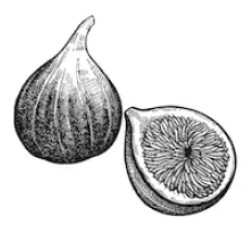
\includegraphics[width=1in,height=1.25in,clip,keepaspectratio]{fig1}}]{Michael Shell}
% Use $\backslash${\tt{begin\{IEEEbiography\}}} and then for the 1st argument use $\backslash${\tt{includegraphics}} to declare and link the author photo.
% Use the author name as the 3rd argument followed by the biography text.
% \end{IEEEbiography}

% \vspace{11pt}

% \bf{If you will not include a photo:}\vspace{-33pt}
% \begin{IEEEbiographynophoto}{John Doe}
% Use $\backslash${\tt{begin\{IEEEbiographynophoto\}}} and the author name as the argument followed by the biography text.
% \end{IEEEbiographynophoto}

\bibliographystyle{IEEEtran}
\bibliography{reference}


\vfill

\end{document}
